\documentclass[12pt,oneside]{report}

% Compile this with XeLaTeX (Overleaf: Menu -> Compiler -> XeLaTeX), not pdfLaTeX:
% the thesis text uses Unicode symbols directly (sigma, rho, en/em dashes are not
% used, but the minus sign U+2212 and Greek letters in running prose are), which
% XeLaTeX's native Unicode handling renders without extra packages or escaping.

% ---- Page geometry (adjust to your university's required margins) ----
\usepackage[a4paper,margin=1in]{geometry}

% ---- Fonts and spacing ----
\usepackage{fontspec}
\setmainfont{TeX Gyre Termes}   % metric-compatible Times New Roman clone; free, bundled with TeX Live
\usepackage{setspace}
\onehalfspacing             % matches the Word draft; \doublespacing or \singlespacing to change

% ---- Tables, figures, links ----
\usepackage{calc}
\usepackage{array}
\usepackage{longtable}
\usepackage{booktabs}
\usepackage{graphicx}
\setkeys{Gin}{width=0.85\linewidth,keepaspectratio}  % default size for every \includegraphics (figures are generated wider than the text column)
\usepackage[hyphens]{url}
\usepackage{microtype}
\usepackage[htt]{hyphenat}  % lets long \texttt{} file paths break inside narrow table cells
\usepackage[colorlinks=true,linkcolor=blue,citecolor=blue,urlcolor=blue]{hyperref}

% ---- Bibliography (natbib: swap \bibliographystyle below for a different citation style) ----
\usepackage{natbib}
\bibliographystyle{apalike}  % apalike reads closest to the Word draft's Chicago author-date style

% Pandoc-generated lists use \tightlist; define it since we assemble chapters
% as fragments rather than through pandoc's own standalone template.
\providecommand{\tightlist}{%
  \setlength{\itemsep}{0pt}\setlength{\parskip}{0pt}}

% ---- Front matter ----
\title{Predictive Market Intelligence for Engineering Proposals in the Video Game Co-Development Industry \\[0.5em]
\large A Design Science Research Study of a Bid-Competitiveness Prediction Pipeline for Virtuos' Engineering Business Unit}
\author{[Your full name]}
\date{[Submission date]}

\begin{document}

\maketitle
\tableofcontents
\listoffigures

\hypertarget{introduction}{%
\chapter{Introduction}\label{introduction}}

\hypertarget{background-and-context}{%
\section{Background and Context}\label{background-and-context}}

Game co-development, the practice of a publisher or platform holder
contracting part or all of a title's production to an external studio,
has grown into a substantial segment of the video game industry.
Industry market-research estimates place the global co-development
services market at approximately USD 4.8 billion in 2025, with
Asia-Pacific holding the largest regional share at an estimated 38.2\%
of revenue \citep{marketintelo2025gamecodev}. These figures come from
vendor market-research reports rather than peer-reviewed sources and
should be read as order-of-magnitude estimates, not precise
measurements; segment definitions vary considerably between research
firms, and comparable reports place narrower slices of the outsourcing
market at under USD 2 billion for the same year. What the estimates
agree on, even allowing for that uncertainty, is that co-development is
a competitive, bid-driven market in which engineering service providers
such as Virtuos routinely compete for a limited number of large,
multi-month contracts against other studios.

For an engineering business unit (BU) operating in this market, each bid
represents a significant commitment of proposal-writing effort,
technical scoping time, and pricing judgement, well before any revenue
is realised. The decision of which opportunities to pursue, how to price
them, and how to shape the proposal to the client's stated and unstated
priorities is, in most engineering-led organisations, made by combining
the business development team's commercial judgement with technical
leads' estimates of feasibility and cost. This is not a criticism
specific to Virtuos: it is the default mode of operation across
professional-services and project-based engineering firms, and it has a
well-documented analogue in enterprise sales, where opportunity
qualification and win-probability estimation have historically relied on
sales representatives' subjective assessment of a deal's likelihood to
close \citep{yan2015sales}.

The consequence of a judgement-based process is not that it performs
badly on average; experienced business development and engineering leads
often have good calibrated intuition. The consequence is that the
judgement is difficult to make consistent across people, difficult to
audit after the fact, and difficult to improve systematically, because
the reasoning behind a ``this bid looks competitive'' assessment is
rarely written down in a form that can be checked against what actually
happened once the bid was won or lost. Over enough bids, the
organisation accumulates a resolved history, Won and Lost outcomes, that
in principle encodes exactly the pattern the team is trying to reason
about by eye: which combinations of client relationship, pricing, team
fit, and competitive context tend to produce a win. In practice, that
history is rarely mined systematically, and the intuitive model stays
implicit, unverified, and non-transferable between people.

\hypertarget{problem-statement}{%
\section{Problem Statement}\label{problem-statement}}

Virtuos' Engineering BU does not currently have a quantitative,
repeatable method for estimating how competitive a given proposal is
likely to be before it is submitted, or for identifying, after the fact,
which factors actually distinguished its won bids from its lost ones.
Bid-level decisions, including whether to pursue an opportunity at all,
how aggressively to price it, and which parts of the technical narrative
to emphasise, are made largely on a manual, gut-feeling basis. This
creates three concrete inefficiencies that motivate this thesis:

\begin{enumerate}
\def\labelenumi{\arabic{enumi}.}
\tightlist
\item
  \textbf{Inconsistent pursuit decisions.} Without a shared,
  data-grounded view of what makes a bid competitive, different business
  development leads may reach different conclusions about the same
  opportunity, and the organisation has no systematic way to reconcile
  those views against historical outcomes.
\item
  \textbf{Pricing left to intuition.} Price positioning relative to the
  market, one of the most consequential and most reversible levers in a
  proposal, is set without a structured view of how price sensitivity
  has actually played out across past bids, by client segment or project
  type.
\item
  \textbf{Missed revenue opportunities.} Opportunities that a
  quantitative read of past patterns would flag as winnable may be
  under-pursued, while resource-intensive proposals for structurally
  weak opportunities may be over-invested, because the only signal
  available is each individual's prior experience.
\end{enumerate}

A machine-learning model trained on the BU's historical bid outcomes,
paired with an explanation method that shows \emph{why} the model
believes a given bid is or is not competitive, offers a way to make the
implicit pattern explicit, check it against what the BU already
believes, and put it in front of decision-makers in a form they can
interrogate rather than simply trust.

\hypertarget{research-aim-and-objectives}{%
\section{Research Aim and
Objectives}\label{research-aim-and-objectives}}

The aim of this thesis is to design, build, and evaluate an end-to-end
decision-support pipeline that predicts the win probability of an
Engineering BU proposal and explains that prediction in terms a
non-technical business stakeholder can act on, and to demonstrate that
pipeline as a working artefact rather than only as a theoretical
proposal.

The specific objectives are to:

\begin{enumerate}
\def\labelenumi{\arabic{enumi}.}
\tightlist
\item
  Define and justify a feature set describing a bid (client relationship
  history, deal origin, pricing position, team and portfolio fit, and
  competitive context) grounded in the Engineering BU's own documented
  hypotheses about what drives competitiveness.
\item
  Build a supervised classification pipeline that predicts the
  probability a proposal is won, following the CRISP-DM process
  \citep{chapman2000crispdm} end to end from data understanding through
  to a working artefact.
\item
  Apply SHAP (SHapley Additive exPlanations) \citep{lundberg2017unified}
  to the trained model to produce both a global ranking of which
  features actually drive its predictions and a per-bid explanation of
  why a specific proposal scores as it does.
\item
  Compare that SHAP-derived ranking systematically against the BU's own
  documented hypotheses about what makes a bid competitive, to surface
  where the two agree and, more importantly, where they diverge.
\item
  Package the pipeline's output as an interactive artefact, a results
  dashboard and a what-if bid scorer, that a BU stakeholder can use
  directly, and evaluate that artefact against the research questions
  below.
\end{enumerate}

\hypertarget{research-questions}{%
\section{Research Questions}\label{research-questions}}

\textbf{RQ1 (Feature Identification).} What bid-level features, drawn
from client relationship history, deal origin, pre-proposal engagement,
pricing position, team and portfolio fit, and competitive context, most
effectively predict a co-development proposal's competitive outcome, and
how does the model's own ranking of those features compare with the
Engineering BU's documented assumptions about what matters?

\textbf{RQ2 (Model Development).} Within a CRISP-DM-structured workflow,
how accurately and how robustly can a supervised classification model
distinguish competitive from uncompetitive proposals under realistic
constraints, specifically a modest sample size, class imbalance toward
losses, and noisy, partially overlapping feature effects, and what does
that accuracy imply about the ceiling on what a purely
historical-pattern model can achieve for this problem?

\textbf{RQ3 (Artefact Demonstration).} How does an interactive,
explanation-driven dashboard, combining aggregate model evaluation,
global and per-bid SHAP explanations, and a live what-if scorer, convert
a trained model's output into decision-support information that an
Engineering BU stakeholder can use and trust, and what does building and
exercising that artefact reveal about the practical requirements for
deploying this kind of tool?

These three research questions correspond, respectively, to the data and
feature-engineering stage of the pipeline, the modelling stage, and the
deployment and human-facing stage, and are addressed in Chapters 4
(Design and Implementation) and 5 (Evaluation) after the methodological
groundwork is laid in Chapter 3.

\hypertarget{significance-of-the-study}{%
\section{Significance of the Study}\label{significance-of-the-study}}

This thesis is positioned as Design Science Research (DSR) in the sense
articulated by Peffers et al. \citep{peffers2007design}: its primary
contribution is a designed, demonstrable artefact that solves a stated
organisational problem, evaluated against that problem, rather than a
purely descriptive or explanatory study. That framing matters for how
the thesis should be read and judged. The contribution is not a claim
about universal truths of what wins video game co-development bids; it
is a validated method, a pipeline that takes a BU's historical bid data
and its documented competitiveness hypotheses and turns them into a
working, explainable prediction tool, together with evidence that the
method behaves correctly and produces decision-relevant output.

Prior work on win-probability modelling in adjacent business domains
supports the premise that this class of problem is tractable with
supervised learning, while also setting realistic expectations for its
limits. Yan et al. \citep{yan2015sales} and Rezazadeh
\citep{rezazadeh2020generalized} both report that enterprise sales
win-propensity models trained on modest, noisy, single-organisation
datasets can meaningfully outperform naive baselines, while cautioning
that B2B datasets are typically small relative to consumer settings,
which constrains achievable accuracy. Zahid et al.
\citep{zahid2021predicting} extend this to tendering specifically,
showing that a multi-class treatment of loss reasons (no bid, client did
not pursue, lost to competition) can add decision-relevant nuance beyond
a flat win and loss label. On the explanation side, Olan et al.
\citep{olan2024enabling} document growing use of SHAP-based
explainability inside supply-chain decision-support systems precisely
because it lets non-technical stakeholders interrogate \emph{why} a
model produced a given output, which is the same requirement this thesis
treats as central to RQ3. This thesis extends that line of work to a
domain, video game co-development bidding, that does not yet have a
published treatment, and does so with an explicit focus on pairing the
predictive model with an interactive artefact rather than reporting
model accuracy alone.

\hypertarget{scope-deviations-from-the-original-proposal-and-limitations}{%
\section{Scope, Deviations from the Original Proposal, and
Limitations}\label{scope-deviations-from-the-original-proposal-and-limitations}}

Three scoping decisions, two of which represent deliberate deviations
from this thesis's original proposal, define what is and is not claimed
here, and are stated plainly up front rather than left for the reader to
discover in later chapters.

\textbf{Synthetic data, not real bid records.} No real, resolved Virtuos
bid data was available for this thesis. The dataset used throughout is
synthetically generated: feature-to-outcome relationships are encoded by
the author from the Engineering BU's documented feature hypotheses, with
added noise, correlation between features, interaction effects, class
imbalance, and label noise so that the data is not trivially learnable
(full detail and justification in Chapter 3 and Appendix A). The
consequence is that this thesis demonstrates that the pipeline correctly
recovers a known, encoded signal under realistic conditions; it is a
validation of the method, not a discovery of what actually wins real
Virtuos bids. Any number reported about feature importance or model
accuracy in Chapters 4 and 5 should be read with that distinction in
mind, and the artefact itself carries this caveat visibly rather than
only in the written thesis.

\textbf{A single gradient-boosted model, not a Random Forest versus
XGBoost comparison.} The original thesis topic specified comparing
Random Forest and XGBoost as candidate classifiers. During
implementation, the pipeline was instead built and evaluated around a
single gradient-boosted tree ensemble (scikit-learn's
\texttt{GradientBoostingClassifier}), paired with a logistic-regression
surrogate used specifically to drive the artefact's interactive scorer
(Chapter 4 explains why a second, linear model was needed for that
component). This is a deliberate narrowing of scope, made to keep the
modelling, explanation, and artefact-building effort proportionate to a
single-semester thesis, and it is treated in Chapter 6 as a limitation
with a concrete recommendation: a Random Forest and XGBoost comparison
is identified there as the most immediately valuable piece of future
work, not discarded as out of scope for the research questions
themselves, since RQ2 is framed around classification accuracy and
robustness rather than around any one algorithm family.

\textbf{An interactive web dashboard, not a Power BI dashboard.} The
original proposal specified Power BI, refreshed through an MLOps
pipeline, as the artefact's delivery mechanism. The delivered artefact
is instead a self-contained, interactive web dashboard (built as HTML,
CSS and JavaScript, with D3.js for charting) embedding both the results
view required by RQ3 and a live, client-side what-if bid scorer,
published both as a shareable Claude Artifact and as a static site
hosted on GitHub Pages. This substitution was made for three practical
reasons, elaborated in Chapter 3: it removes a Power BI Desktop/Service
licensing dependency that would otherwise gate reviewers' ability to
open the artefact at all; it allows the scorer's probability calculation
to run as an exact, auditable client-side computation rather than
through a Power BI data-refresh cycle; and it kept iteration speed
compatible with building the artefact and the thesis in parallel. The
trade-off this incurs, namely that Power BI's native enterprise
deployment, row-level security, and scheduled-refresh features are not
demonstrated, is treated explicitly as a limitation in Chapter 6,
alongside a concrete description of what porting the current pipeline's
output to Power BI would involve.

Beyond these three points, the thesis is scoped to a single business
unit (Engineering) within a single organisation (Virtuos), to the
specific feature set described in Chapter 3, and to a proof-of-concept
level of artefact maturity: production deployment considerations such as
authentication, audit logging, and integration with a live CRM are out
of scope.

\hypertarget{structure-of-the-thesis}{%
\section{Structure of the Thesis}\label{structure-of-the-thesis}}

The remainder of this thesis is organised as follows. \textbf{Chapter 2}
reviews the literature on machine learning for bid- and
sales-opportunity prediction, explainable AI and SHAP in business
decision support, and Design Science Research and CRISP-DM as
methodological frameworks, situating this thesis's contribution relative
to that work. \textbf{Chapter 3} sets out the methodology in full: the
Design Science Research process followed, the CRISP-DM stages as applied
to this project, the synthetic data generation methodology and its
justification, and a fuller account of the three scoping deviations
introduced in Section 1.6. \textbf{Chapter 4} describes the design and
implementation of the pipeline and artefact: the feature engineering,
the model training and SHAP explanation pipeline, and the architecture
of the interactive dashboard and scorer. \textbf{Chapter 5} reports the
evaluation: quantitative model performance (AUC, Brier score, precision,
recall, F1), the SHAP-versus-hypothesis comparison, and a qualitative
assessment of the artefact against RQ3. \textbf{Chapter 6} discusses
what the results mean, the limitations introduced by the synthetic-data
and scoping decisions, and the threats to validity. \textbf{Chapter 7}
concludes with a summary of the contribution and a concrete set of
recommendations for future work, led by moving the pipeline onto real
bid data. Appendices provide the full synthetic-data generation
methodology, the complete feature glossary used throughout the artefact,
and selected code listings.

\hypertarget{literature-review}{%
\chapter{Literature Review}\label{literature-review}}

This chapter reviews four bodies of work that this thesis draws on:
machine learning applied to sales- and bid-opportunity prediction;
tree-based ensemble classifiers and the trade-offs between them;
explainable AI, specifically SHAP, as a mechanism for turning a model's
output into something a business stakeholder can act on; and Design
Science Research together with CRISP-DM as the methodological
scaffolding for building and evaluating the artefact. The chapter closes
by identifying the specific gap this thesis addresses: the combination
of these four threads has not, to the author's knowledge, been applied
to bid-competitiveness prediction in the video game co-development
industry.

\hypertarget{machine-learning-for-sales-and-bid-opportunity-prediction}{%
\section{Machine Learning for Sales and Bid-Opportunity
Prediction}\label{machine-learning-for-sales-and-bid-opportunity-prediction}}

Predicting whether a commercial opportunity will be won is a
well-established problem in enterprise sales analytics, and the closest
published analogues to this thesis's problem come from that literature
rather than from the game industry specifically. Yan et al.
\citep{yan2015sales}, working with IBM Research on data from a top-500
enterprise, frame the task as win-propensity prediction: estimating the
probability that an open sales opportunity will close within a given
time window. Their central methodological point is one this thesis
inherits directly: business-to-business (B2B) opportunity data is small
relative to consumer-scale datasets, noisy, and drawn from a market that
shifts over the period the data covers, all of which constrain how much
accuracy any model can realistically achieve and argue against treating
a single point accuracy figure as the measure of success. The same
constraint applies, likely more severely, to a single engineering BU's
resolved bid history, which is the premise this thesis's synthetic-data
approach is built to test under controlled conditions (Chapter 3).

Rezazadeh \citep{rezazadeh2020generalized} reports a generalised
ensemble-modelling workflow for B2B sales prediction built on Microsoft
Azure Machine Learning and evaluated on a consulting firm's historical
opportunity data, with a data-enrichment and feature-engineering stage
treated as integral to the pipeline rather than as a preprocessing
afterthought. This supports the structural choice made in this thesis's
own pipeline (Chapter 4) to treat feature engineering as its own
CRISP-DM stage rather than folding it into model training. Zahid et al.
\citep{zahid2021predicting} extend the basic win/loss framing by
splitting losses into three distinct classes, no bid, customer did not
pursue, and lost to competition, and report 85\% accuracy with an
average AUC of 0.94 for B2B tendering data once class imbalance is
handled. Their multi-class treatment is a useful pointer for future work
(Chapter 7): the dataset generator built for this thesis already
distinguishes Won from Lost but, consistent with their finding that loss
\emph{reasons} carry separate decision-relevant information, does not
yet separate ``we chose not to bid'' from ``we bid and lost,'' a
distinction the Engineering BU would likely want in a production version
of this tool.

Two methodological lessons recur across this literature and shape how
this thesis evaluates its own model in Chapter 5. First, raw accuracy is
a poor summary statistic for a class-imbalanced win/loss problem,
because a model that always predicts the majority class (``Lost'') can
post misleadingly high accuracy while never identifying a single win; He
and Garcia \citep{he2009learning}, in their survey of learning from
imbalanced data, make the same point in general terms and recommend
threshold-independent measures such as the area under the ROC curve
(AUC) and probability-calibration measures such as the Brier score as
more informative summaries, both of which this thesis reports alongside
accuracy for that reason. Second, every one of these papers works with
real but \emph{confidential} organisational data that cannot be
published or independently re-examined, which is a structural problem
for reproducibility in this research area generally and is one of the
reasons, discussed fully in Chapter 3, that this thesis instead builds
and publishes a synthetic dataset whose generating process is fully
disclosed.

\hypertarget{tree-based-ensemble-classifiers-for-tabular-prediction-problems}{%
\section{Tree-Based Ensemble Classifiers for Tabular Prediction
Problems}\label{tree-based-ensemble-classifiers-for-tabular-prediction-problems}}

Bid-level features of the kind described in Section 1.3, a mixture of
categorical fields (client segment, project type), ordinal fields
(relationship history), and continuous fields (price position, effort),
is a textbook tabular-data classification problem, and the dominant
family of models for this problem class remains tree-based ensembles
rather than deep learning. Breiman's Random Forest
\citep{breiman2001random} averages many decision trees, each trained on
a bootstrap-resampled subset of the data and a random subset of features
at each split, trading a small amount of bias for a substantial
reduction in variance relative to a single tree; it is robust to
irrelevant features, requires comparatively little hyperparameter
tuning, and handles the mix of feature types in this problem natively,
which is why it was specified as a candidate algorithm in this thesis's
original proposal (Section 1.6).

Gradient boosting, introduced by Friedman \citep{friedman2001greedy},
takes a different approach to the same underlying idea of combining many
weak learners: rather than averaging independently trained trees, it
fits each new tree to the residual error of the ensemble built so far,
so that the ensemble is built as a stagewise, additive approximation
that directly minimises a chosen loss function. XGBoost
\citep{chen2016xgboost} is an engineering-optimised implementation of
gradient boosting that adds regularisation terms to the objective, a
more careful treatment of missing values, and substantial training-speed
improvements, and was the second algorithm specified in this thesis's
original proposal. In practice, Random Forest and gradient-boosted
variants (including XGBoost and scikit-learn's own
\texttt{GradientBoostingClassifier}) tend to perform comparably on
small-to-medium tabular datasets, with the gap between them typically
smaller than the gap between either and a well-tuned linear model on
genuinely non-linear data, and smaller again than the variance
introduced by dataset size and noise. This thesis's choice to build
around scikit-learn's \texttt{GradientBoostingClassifier}, a direct
implementation of Friedman's \citeyearpar{friedman2001greedy} algorithm,
rather than running the originally proposed Random Forest-versus-XGBoost
comparison, is a scoping decision made for the reasons given in Section
1.6, not a claim that gradient boosting is definitively superior for
this problem; Chapter 7 identifies the comparison as the most
immediately valuable piece of future work precisely because the
literature does not settle the question in advance.

A second, independent reason tree ensembles rather than linear models
are the right default for this problem is that bid competitiveness
plausibly involves interaction effects rather than a purely additive
combination of features, for example a weak project-portfolio match may
matter far more for a brand-new client than for a client with a strong
prior relationship. Tree-based models capture such interactions natively
through their split structure, where a linear or logistic model would
require those interaction terms to be specified by hand in advance. This
consideration directly motivated the synthetic data generator's design
(Chapter 3), which deliberately encodes several such interaction effects
so that the modelling pipeline has a genuine reason to need a non-linear
learner rather than a toy problem a linear model could solve equally
well.

\hypertarget{explainable-ai-and-shap-in-business-decision-support}{%
\section{Explainable AI and SHAP in Business Decision
Support}\label{explainable-ai-and-shap-in-business-decision-support}}

A model that outputs a win probability without any account of \emph{why}
is of limited use to a bid-review meeting: a business development lead
who is told ``62\%'' and nothing else has no way to check the number
against what they already know, challenge it, or act differently because
of it. This is the motivation for pairing the predictive model with an
explanation method rather than treating prediction as the end goal,
which is the premise behind RQ3 (Section 1.4).

SHAP (SHapley Additive exPlanations), introduced by Lundberg and Lee
\citep{lundberg2017unified}, addresses this by adapting the Shapley
value, a concept from cooperative game theory that fairly distributes a
total payoff among players based on their marginal contribution across
all possible coalitions, to the problem of attributing a model's
prediction to its input features. For a single prediction, SHAP assigns
each feature a signed contribution such that the contributions sum
exactly to the difference between that prediction and the model's
average prediction across the training data; this additive,
exact-decomposition property is what distinguishes it from earlier
feature-importance methods, which typically report only a global ranking
with no guarantee that per-instance explanations are internally
consistent. For tree ensembles specifically, Lundberg and Lee's TreeSHAP
algorithm computes these exact Shapley values in polynomial rather than
exponential time, which is what makes SHAP computationally practical for
the hundreds of predictions this thesis's pipeline explains (Chapter 4)
rather than only a handful.

Published applications of SHAP in business decision-support contexts
remain comparatively recent but are growing. Olan et al.
\citep{olan2024enabling} review the use of explainable AI, with SHAP as
a central example, inside supply-chain decision-support systems, and
report that explainability has been instrumental in enabling
organisations to act on model output with confidence rather than
treating it as an opaque score; their framing of SHAP's role, making a
model's reasoning available for human review rather than only its
output, is the same framing this thesis adopts for RQ3 and for the
dashboard design in Chapter 4. The pattern observed across this
literature, including Olan et al.'s own account, is that published SHAP
applications concentrate in a small number of domains (credit risk,
supply chains, retail cross-selling, and clinical prediction) and that
bid- or proposal-level win prediction in any industry, let alone video
game co-development specifically, does not yet appear in this
literature. That absence is itself part of the gap this thesis
addresses.

This thesis's use of SHAP serves two distinct purposes that the
literature above generally treats separately. The first is per-bid
explanation: showing a decision-maker which features pushed a specific
proposal's predicted win probability up or down, which is the direct
analogue of Olan et al.'s supply-chain use case. The second, more
specific to this thesis's design, is using SHAP's \emph{global}
feature-ranking output as a structured object to compare against the
Engineering BU's own documented hypotheses about what drives
competitiveness (RQ1), turning the explanation method into an instrument
for checking a model against domain expertise rather than only for
explaining the model's output to an end user. This comparative use of
SHAP, model-derived ranking against a priori domain hypotheses, is the
thesis's clearest point of methodological contribution relative to the
reviewed literature, and is developed fully in Chapter 3's discussion of
the hypothesis-comparison design and evaluated in Chapter 5.

\hypertarget{design-science-research-and-crisp-dm-as-methodological-frameworks}{%
\section{Design Science Research and CRISP-DM as Methodological
Frameworks}\label{design-science-research-and-crisp-dm-as-methodological-frameworks}}

This thesis is framed as Design Science Research (DSR), a research
paradigm concerned with building and evaluating artefacts that address
an identified organisational problem, as distinct from behavioural
research, which seeks to explain or predict phenomena without building
anything. Hevner et al. \citep{hevner2004design} set out seven
guidelines for DSR in information systems research, of which three are
directly load-bearing for how this thesis is structured: the research
must produce a viable, purposeful artefact (Guideline 1); the artefact
must be rigorously evaluated to demonstrate its utility (Guideline 3);
and the research process itself, not only its output, must be clearly
and repeatably documented (Guideline 7). Chapters 4 and 5 of this thesis
are organised directly around the first two of these guidelines,
describing the artefact's construction and then its evaluation as
distinct, sequential activities, and the full disclosure of the
synthetic-data generation process in Chapter 3 and Appendix A is this
thesis's response to the third.

Peffers et al. \citep{peffers2007design} operationalise DSR into six
concrete process steps: problem identification and motivation,
definition of objectives for a solution, design and development,
demonstration, evaluation, and communication. This thesis follows that
sequence structurally: Chapter 1 covers problem identification and
motivation and the definition of objectives; Chapter 3 (methodology) and
Chapter 4 (design and implementation) cover design and development;
Chapter 4's description of the working dashboard and scorer constitutes
demonstration; Chapter 5 covers evaluation; and this thesis document
itself, together with the published artefact, is the communication step.
Peffers et al.'s framework explicitly allows for a ``problem-centred''
entry point, where the research begins from a known organisational
problem rather than from an opportunity noticed in existing technology,
which matches how this thesis originated, from the Engineering BU's
stated difficulty in Section 1.2, rather than from a novel algorithmic
technique in search of an application.

Within the design and development step, CRISP-DM (Cross-Industry
Standard Process for Data Mining) \citep{chapman2000crispdm} provides
the specific process model this thesis follows for the
data-and-modelling portion of the work. CRISP-DM structures a data
mining project into six phases, business understanding, data
understanding, data preparation, modelling, evaluation, and deployment,
applied iteratively rather than strictly linearly. Schröer et al.'s
systematic review of CRISP-DM applications \citep{schroer2021systematic}
finds it remains the de facto standard process model across a wide range
of application domains more than two decades after its publication,
which supports treating it as the appropriate choice here rather than a
more recent alternative; their review also notes that most published
applications adapt CRISP-DM's phases to their specific domain rather
than applying it unmodified, which this thesis does explicitly in
Chapter 3 by mapping each CRISP-DM phase onto a concrete, named stage of
the pipeline described in Chapter 4.

Using DSR and CRISP-DM together, as this thesis does, is a natural
pairing rather than a redundant one: DSR provides the outer research
framework that justifies building an artefact and specifies how it must
be evaluated as a contribution to knowledge, while CRISP-DM provides the
inner, domain-specific process discipline for the data mining work that
sits inside that artefact's ``design and development'' step. Chapter 3
sets out exactly how the two are nested in this thesis's own process.

\hypertarget{synthesis-and-identified-gap}{%
\section{Synthesis and Identified
Gap}\label{synthesis-and-identified-gap}}

Reading these four bodies of work together situates this thesis
precisely. The sales- and tendering-prediction literature
\citep{yan2015sales, zahid2021predicting, rezazadeh2020generalized}
establishes that win-probability prediction from historical opportunity
data is a tractable, previously validated problem class, but every
published instance works with confidential, unpublished organisational
data and, as far as this review found, none addresses the video game
co-development industry specifically. The tree-ensemble literature
\citep{breiman2001random, friedman2001greedy, chen2016xgboost}
establishes Random Forest and gradient boosting as the appropriate
default model family for this kind of tabular, mixed-type,
interaction-rich feature set, without settling which specific variant is
best in advance of testing on the data at hand. The explainability
literature \citep{lundberg2017unified, olan2024enabling} establishes
SHAP as a credible, increasingly adopted mechanism for making a
business-facing model's output actionable, but has not, to this review's
knowledge, been applied to compare a trained model's findings
systematically against a business unit's own documented a priori
hypotheses, which is precisely what RQ1 does. The methodology literature
\citep{hevner2004design, peffers2007design, chapman2000crispdm, schroer2021systematic}
provides a well-established process for building and evaluating exactly
this kind of artefact, but offers no domain-specific guidance for
proposal bidding in creative-industry outsourcing.

The gap this thesis addresses, then, is not a gap in any one of these
four literatures individually, each is mature on its own terms, but the
absence of their combination applied to this specific, previously
unstudied domain: a DSR-grounded, CRISP-DM-structured pipeline that
predicts bid competitiveness for video game co-development proposals,
uses SHAP both to explain individual predictions and to systematically
check the model against the Engineering BU's own stated assumptions, and
packages the result as a working, demonstrable artefact rather than a
modelling exercise reported only in tables. Chapter 3 now turns to the
methodology used to fill that gap.

\hypertarget{methodology}{%
\chapter{Methodology}\label{methodology}}

This chapter sets out how the thesis was carried out: the Design Science
Research process followed, how CRISP-DM structures the
data-and-modelling work inside that process, the full methodology and
justification for the synthetic dataset the pipeline is trained and
evaluated on, and a detailed account of the three scoping decisions
introduced briefly in Section 1.6. The chapter closes with the tools and
technologies used and a statement of the evaluation approach that
Chapter 5 then applies.

\hypertarget{overarching-framework-design-science-research}{%
\section{Overarching Framework: Design Science
Research}\label{overarching-framework-design-science-research}}

This thesis follows the six-step Design Science Research process set out
by Peffers et al. \citep{peffers2007design}, entered at the
problem-centred initiation point since the work began from a stated
organisational problem (Section 1.2) rather than from a technology
opportunity. Table 3.1 maps each DSR step to where it is addressed in
this thesis.

\begin{longtable}[]{@{}
  >{\raggedright\arraybackslash}p{(\columnwidth - 4\tabcolsep) * \real{0.3333}}
  >{\raggedright\arraybackslash}p{(\columnwidth - 4\tabcolsep) * \real{0.3333}}
  >{\raggedright\arraybackslash}p{(\columnwidth - 4\tabcolsep) * \real{0.3333}}@{}}
\toprule\noalign{}
\begin{minipage}[b]{\linewidth}\raggedright
DSR step (Peffers et al.~2007)
\end{minipage} & \begin{minipage}[b]{\linewidth}\raggedright
How it is addressed
\end{minipage} & \begin{minipage}[b]{\linewidth}\raggedright
Thesis location
\end{minipage} \\
\midrule\noalign{}
\endhead
\bottomrule\noalign{}
\endlastfoot
1. Problem identification and motivation & The Engineering BU's manual,
inconsistent bid-pursuit and pricing process, and the gap between
resolved bid history and systematic use of it & Section 1.1, 1.2 \\
2. Definition of objectives for a solution & Five concrete objectives:
feature identification, CRISP-DM pipeline, SHAP explanation, hypothesis
comparison, interactive artefact & Section 1.3 \\
3. Design and development & Synthetic data generation, feature
engineering, model training, SHAP pipeline, dashboard and scorer
construction & This chapter; Chapter 4 \\
4. Demonstration & The working dashboard and scorer, exercised against
realistic example bids & Chapter 4, Section 4.4 \\
5. Evaluation & Quantitative model performance, SHAP-vs-hypothesis
comparison, qualitative artefact assessment against RQ3 & Chapter 5 \\
6. Communication & This thesis document and the published, shareable
artefact & Throughout; artefact links in Chapter 4 \\
\end{longtable}

Hevner et al.'s \citep{hevner2004design} guideline that the research
process itself be rigorously and repeatably documented (their Guideline
7) is addressed concretely by making every stage of the pipeline, from
the synthetic data generator through to the published dashboard,
available as runnable, version-controlled source code rather than
described only in prose; Appendix C lists the complete set of scripts
and where each DSR and CRISP-DM step is implemented.

\hypertarget{the-data-mining-process-crisp-dm}{%
\section{The Data Mining Process:
CRISP-DM}\label{the-data-mining-process-crisp-dm}}

Within the ``design and development'' DSR step, the data-and-modelling
portion of the work follows CRISP-DM \citep{chapman2000crispdm}, adapted
to this project in the manner Schröer et al.
\citep{schroer2021systematic} find typical of published CRISP-DM
applications: the six phases are followed in substance, iteratively
rather than strictly linearly, with each phase mapped onto a concrete,
named artefact rather than treated as an abstract checklist item.

\textbf{Business understanding.} The business problem (Section 1.2) was
translated into a supervised binary classification problem: given a
bid's features at the time it is submitted, predict whether the outcome
will be Won or Lost. The Engineering BU's documented feature hypotheses,
its own prior, qualitative beliefs about what makes a bid competitive,
were treated as the business-understanding artefact this phase is meant
to produce, and are used twice downstream: first as the basis for the
synthetic data generator's encoded relationships (next section), and
second as the comparison point for the trained model's SHAP ranking
(RQ1).

\textbf{Data understanding.} Because no real, resolved bid data was
available (Section 1.6), this phase consisted of specifying the feature
set itself, thirteen fields spanning client relationship history, deal
origin, pre-proposal engagement, incumbency position, effort, price
position, requirement coverage, portfolio fit, geographic/timezone fit,
security credentials, and the number of competing bidders, and
establishing plausible marginal distributions and realistic missingness
patterns for each, so that the resulting dataset would read as a
plausible bid log rather than an obviously synthetic grid of round
numbers.

\textbf{Data preparation.} The thirteen features were encoded for
modelling (one-hot encoding for categorical fields, median imputation
for missing numeric values, most-frequent imputation for missing
categorical values), and the dataset was split 75/25 into training and
held-out test sets, stratified on the outcome label to preserve the
roughly 30\% win rate in both splits (Chapter 4, Section 4.2 gives full
implementation detail).

\textbf{Modelling.} A gradient-boosted tree ensemble (scikit-learn's
\texttt{GradientBoostingClassifier}, implementing Friedman's
\citeyearpar{friedman2001greedy} algorithm) was trained on the prepared
training data, with hyperparameters (tree depth, learning rate, minimum
samples per leaf, subsampling rate) selected to balance fit against the
overfitting risk that a dataset of 500 rows and thirteen features
otherwise carries. A second, linear logistic-regression model was also
trained on the full dataset specifically to support the artefact's
interactive scorer; Section 3.4 explains why a second model was needed
for that component rather than reusing the gradient-boosted model
directly.

\textbf{Evaluation.} The gradient-boosted model was evaluated on the
held-out test set using AUC, the Brier score, and a confusion matrix at
the default 0.5 threshold, and separately using 5-fold stratified
cross-validation across the full dataset for a more stable accuracy
estimate. SHAP values were computed for every bid in the dataset and
aggregated into a global feature-importance ranking, which was then
compared quantitatively (via Spearman rank correlation) against the BU's
documented hypothesis ranking. Full results are reported in Chapter 5.

\textbf{Deployment.} The trained model's output, performance metrics,
SHAP values, the hypothesis comparison, and the logistic surrogate's
coefficients, was exported as a single structured results file and used
to drive the interactive dashboard and scorer described in Chapter 4,
published as a shareable web artefact rather than deployed into a live
production system, consistent with this thesis's proof-of-concept scope
(Section 1.6).

\hypertarget{synthetic-data-full-methodology-and-justification}{%
\section{Synthetic Data: Full Methodology and
Justification}\label{synthetic-data-full-methodology-and-justification}}

No empirical, resolved Virtuos bid records were available at the time
this thesis was carried out. Rather than treat this as a blocking
constraint, the data generation step was designed as a deliberate
validation exercise: a synthetic dataset in which the relationships
between features and the Won/Lost outcome are \emph{encoded by the
author}, derived from the Engineering BU's documented feature hypotheses
rather than from the author's own preference or from any real
practitioner data, so that the entire downstream pipeline, modelling,
SHAP, hypothesis comparison, artefact, can be exercised and checked
against a known, recoverable signal before any real data is available.

The claim this validates is narrow and stated explicitly: \emph{the
pipeline correctly recovers feature-outcome relationships that were
encoded from the Engineering BU's documented hypotheses, under realistic
noise}. Because the data generator's weights come from the same
hypotheses the trained model's SHAP ranking is later compared against,
agreement between the two is expected by construction and is not
independent evidence about real Virtuos bids; it is evidence that the
\emph{method} works. This distinction is maintained throughout this
thesis and is repeated here because it is the single most important
methodological caveat in the entire study.

\hypertarget{design-principles-against-trivial-circularity}{%
\subsection{Design Principles Against Trivial
Circularity}\label{design-principles-against-trivial-circularity}}

A generator that encodes a clean, deterministic rule (for example, ``win
if and only if price is below benchmark and relationship history is
positive'') would let any model, including a trivial one, achieve
near-perfect accuracy, which would demonstrate nothing about the
pipeline's ability to recover a \emph{realistically noisy} signal. Six
design principles were applied specifically to avoid this:

\begin{enumerate}
\def\labelenumi{\arabic{enumi}.}
\tightlist
\item
  \textbf{Noisy logistic outcome.} The win probability for each bid is a
  logistic function of a latent score, computed as a weighted sum of
  encoded feature effects, plus independent Gaussian noise (σ ≈ 1.25)
  added to that latent score before the logistic transform. The model
  therefore cannot achieve near-100\% accuracy even if it recovers every
  encoded relationship exactly.
\item
  \textbf{Label noise.} Approximately 5\% of outcomes are flipped after
  the logistic draw, mimicking the mislabelled or genuinely surprising
  results that occur in real bid logs (an unusually priced bid that wins
  anyway, a strong proposal lost to an unmodelled factor).
\item
  \textbf{Correlated features.} Features are drawn with realistic
  correlations rather than independently: inbound deal origin is more
  likely given a prior good relationship; pre-proposal engagement is
  more likely given either inbound origin or a prior good relationship;
  price position is correlated with project effort (larger engagements
  receive a modest discount).
\item
  \textbf{Interaction effects.} Three non-additive interactions are
  deliberately encoded: a weak portfolio match penalises a brand-new
  client far more than a repeat client; security credentials matter
  substantially more for AAA-publisher and platform-holder clients than
  for other segments; and indie-studio clients are more price-sensitive,
  so overpricing carries an extra penalty specific to that segment. A
  purely linear model cannot fully capture these, which motivates the
  use of a tree-based learner (Section 2.2) rather than only a linear
  baseline.
\item
  \textbf{Class imbalance.} The intercept of the logistic model is
  calibrated so the overall win rate lands close to 30\%, matching a
  realistic bid log rather than an artificially balanced 50/50 split,
  and forcing the pipeline to handle the imbalance explicitly in its
  evaluation (Section 2.1, He and Garcia \citep{he2009learning}) rather
  than benefiting from a favourable class balance it would not have on
  real data.
\item
  \textbf{Missing values.} Values are set to missing at random for three
  fields (pre-proposal engagement, requirement coverage, and number of
  competing bidders) at rates of 5 to 8\%, so the pipeline's imputation
  step is genuinely exercised rather than trivially unnecessary.
\end{enumerate}

\hypertarget{a-deliberately-noteworthy-encoded-pattern}{%
\subsection{A Deliberately Noteworthy Encoded
Pattern}\label{a-deliberately-noteworthy-encoded-pattern}}

One relationship is encoded counter-intuitively on purpose, to give the
pipeline something genuinely non-obvious to recover rather than only
confirming an expected monotonic pattern. Relationship history is
modelled on a four-point ordinal scale (new client; prior client whose
delivery went poorly; prior client whose delivery was neutral; prior
client whose delivery went well), and the ``prior client, delivery went
poorly'' level is encoded as \emph{worse} for win probability than a
brand-new client, not simply less good than a positive prior
relationship. A model, and a SHAP analysis, that correctly separates
``prior, poor delivery'' from ``prior, good delivery'' rather than
collapsing all repeat business into a single positive effect
demonstrates that the pipeline captures a nuance a naive binary ``is
this a repeat client?'' feature would miss entirely. Chapter 5 reports
whether this pattern was in fact recovered.

\hypertarget{feature-set}{%
\subsection{Feature Set}\label{feature-set}}

Because synthetic generation removes the constraint of ``was this ever
actually logged,'' the feature set used is somewhat richer than a BU's
real historical records might currently capture. Thirteen features were
generated: client segment, project type, relationship history (the
four-point ordinal scale above, with prior delivery outcome folded in),
deal origin (inbound or outbound), pre-proposal engagement, incumbency
position (greenfield, defending existing work, or displacing a
competitor), effort in person-months, price position relative to
benchmark, requirement coverage, portfolio similarity,
geographic/timezone fit, security credentials, and the number of
competing bidders. The last of these, number of competing bidders,
carries an explicit caveat that is maintained throughout this thesis: in
a real deployment, this figure is frequently known only \emph{after} the
bid decision is made, which makes it a leakage risk if it were available
to the model at training time but not at genuine prediction time. It is
retained here for completeness, since the full set of the BU's
documented hypotheses includes it, but is flagged wherever it appears,
and a real-data implementation of this pipeline should either verify it
is genuinely known at bid time or demote it to analysis-only use
(Chapter 7).

\hypertarget{validation-that-the-data-is-non-trivial}{%
\subsection{Validation That the Data Is
Non-Trivial}\label{validation-that-the-data-is-non-trivial}}

Before any downstream modelling, a simple logistic-regression ceiling
check was run directly on the generated data: a 5-fold cross-validated
logistic regression achieves an AUC of approximately 0.72 on this
dataset. This figure matters as a sanity check in both directions. An
AUC far below this (near 0.5) would indicate the encoded signal was too
weak or too noisy to be learnable at all; an AUC very close to 1.0 would
indicate the data was trivially circular, learnable by any model
regardless of its capability. An AUC around 0.7 to 0.75 for a simple
linear baseline indicates a dataset with real, recoverable signal that
is neither trivial nor unlearnable, exactly the design goal. Chapter 5
compares the gradient-boosted model's own performance against this
baseline.

\hypertarget{the-three-scoping-deviations-in-full}{%
\section{The Three Scoping Deviations, in
Full}\label{the-three-scoping-deviations-in-full}}

Section 1.6 stated three scoping decisions briefly; this section gives
the full reasoning for the two that represent deliberate deviations from
the thesis's original proposal.

\hypertarget{deviation-1-a-single-gradient-boosted-model-instead-of-a-random-forest-versus-xgboost-comparison}{%
\subsection{Deviation 1: A Single Gradient-Boosted Model Instead of a
Random Forest-versus-XGBoost
Comparison}\label{deviation-1-a-single-gradient-boosted-model-instead-of-a-random-forest-versus-xgboost-comparison}}

The original proposal specified comparing Random Forest and XGBoost as
candidate classifiers (RQ2). The delivered pipeline instead trains and
evaluates a single gradient-boosted ensemble, scikit-learn's
\texttt{GradientBoostingClassifier}, a direct implementation of
Friedman's \citeyearpar{friedman2001greedy} algorithm and a close
methodological relative of XGBoost \citep{chen2016xgboost} without that
library's additional engineering optimisations. Three considerations
drove this narrowing. First, proportionate effort: a rigorous Random
Forest-versus-XGBoost comparison, properly tuned and validated, is
itself a substantial piece of modelling work, and given the
single-semester scope of this thesis, that effort was judged better
spent on the SHAP explanation pipeline and the interactive artefact,
which directly address RQ1 and RQ3 and were judged more central to the
thesis's DSR contribution (an explainable, demonstrable decision-support
tool) than an algorithm bake-off would be. Second, the literature
reviewed in Section 2.2 indicates that Random Forest and
gradient-boosted variants typically perform comparably on tabular data
of this size and type, with the gap between them generally smaller than
the variance introduced by dataset size, noise, and feature engineering
choices; the specific choice of ensemble family was judged less
consequential to this thesis's research questions than the
explainability and artefact-design work that those questions actually
hinge on. Third, SHAP's TreeSHAP algorithm \citep{lundberg2017unified}
applies natively and efficiently to gradient-boosted trees, which kept
the explanation pipeline (central to RQ1 and RQ3) straightforward to
implement correctly.

This is treated as a limitation, not a methodological equivalence claim:
RQ2 as stated in Section 1.4 asks about classification accuracy and
robustness under CRISP-DM generally, not about any one named algorithm,
so the research question itself is still answered by the work as
delivered, but the answer is narrower than originally scoped. Chapter 6
revisits this as a threat to validity, and Chapter 7 identifies the
comparison as the single most valuable, well-defined piece of future
work, precisely because the synthetic dataset and evaluation harness
built for this thesis already make that comparison straightforward to
run.

\hypertarget{deviation-2-an-interactive-web-dashboard-instead-of-power-bi}{%
\subsection{Deviation 2: An Interactive Web Dashboard Instead of Power
BI}\label{deviation-2-an-interactive-web-dashboard-instead-of-power-bi}}

The original proposal specified Power BI, refreshed through an MLOps
pipeline using Power BI's APIs, as the artefact's delivery mechanism.
The delivered artefact is an interactive web dashboard, built as
self-contained HTML, CSS, and JavaScript with D3.js for charting,
published both as a shareable Claude Artifact and as a static site. This
substitution was made for three reasons, each with a direct bearing on
RQ3's requirement that the artefact be demonstrable and usable.

First, access. A Power BI dashboard requires reviewers, a thesis
committee, and the Engineering BU's own stakeholders to have Power BI
Desktop or an appropriately licensed Power BI Service account to open it
at all; a web dashboard requires only a browser, which removes a real
access barrier for anyone evaluating or using the artefact, including
during the thesis defence itself.

Second, exactness of the interactive scorer. RQ3 calls for a what-if
scorer a stakeholder can use directly, and the design goal for that
scorer (Section 4.4) was that every factor it displays be an
\emph{exact}, not approximated, contribution to the predicted
probability, computed live as the user adjusts a bid's features. A Power
BI dashboard built against a scheduled data refresh is well suited to
displaying precomputed model output, but is not naturally suited to
running a live, client-side probability calculation in response to user
input; building the scorer as a logistic-regression surrogate evaluated
directly in JavaScript (Section 4.4 explains the surrogate-model choice)
was more straightforward and more exactly auditable as a web artefact
than as a Power BI report.

Third, iteration speed. Building the pipeline, the artefact, and this
thesis in parallel over a single semester favoured a tool with a short
edit-preview-publish cycle; the web dashboard could be revised and
republished within the same working session the underlying model or data
changed, without a separate data-refresh or publish step.

The resulting trade-off is real and is stated plainly rather than
minimised: Power BI's native enterprise deployment model, including
row-level security, scheduled automatic refresh against a live data
source, and integration into an organisation's existing Power BI
workspace alongside other BU reporting, is not demonstrated by this
artefact. Chapter 6 discusses this trade-off as a limitation, and
Appendix B sets out concretely what porting the current pipeline's
output (the structured results file described in the Deployment phase
above) to a Power BI report would involve, since the pipeline was
deliberately built to produce that output as a portable, self-contained
file rather than in a format tied to the web dashboard specifically.

\hypertarget{scoping-decision-3-single-business-unit-proof-of-concept-maturity}{%
\subsection{Scoping Decision 3: Single Business Unit, Proof-of-Concept
Maturity}\label{scoping-decision-3-single-business-unit-proof-of-concept-maturity}}

The third scoping point from Section 1.6, restated here for completeness
rather than as a deviation, is that the thesis is deliberately bounded
to a single business unit within a single organisation and to
proof-of-concept artefact maturity. Production concerns, including
authentication, audit logging, integration with a live CRM or
bid-tracking system, and ongoing model retraining and monitoring, are
explicitly out of scope. This is not a deviation from the original
proposal, which was itself scoped to the Engineering BU, but is stated
here because it bears directly on how Chapter 5's evaluation and Chapter
7's future-work recommendations should be read: this thesis evaluates
whether the pipeline and artefact \emph{work correctly as designed}, not
whether they are production-ready.

\hypertarget{tools-and-technologies}{%
\section{Tools and Technologies}\label{tools-and-technologies}}

The pipeline and artefact were built with Python 3 for data generation
and modelling (NumPy and pandas for data handling, scikit-learn for the
gradient-boosted and logistic-regression models and for cross-validation
and preprocessing utilities, and the \texttt{shap} package for TreeSHAP
explanation), Git for version control of every stage of the pipeline and
of this thesis document itself, and HTML, CSS, JavaScript, and D3.js for
the interactive dashboard and scorer. Pandoc, driven from Markdown
chapter files and a BibTeX reference list, was used to produce this
thesis document, so that chapter text, like the pipeline code, is
version-controlled and diffable rather than held only in binary form.

The static figures reproduced in this thesis (Chapters 4 and 5) are
generated by a dedicated script, \texttt{thesis/make\_figures.py}, using
Matplotlib, rather than drawn by hand or exported once and then edited.
This script reads \texttt{outputs/model\_results.json}, the same file
the pipeline's interactive dashboard reads from, so a figure in this
thesis and the corresponding chart a reader sees in the live dashboard
are two renderings of the same underlying numbers rather than
independently maintained artefacts that could silently drift apart after
a future pipeline run. This follows the same reproducibility principle
Hevner et al.'s \citeyearpar{hevner2004design} seventh guideline calls
for (Section 3.1): re-running \texttt{python3\ thesis/make\_figures.py}
after any change to the model or the data regenerates every figure in
this thesis from the updated results automatically, with no manual
charting step for a future author or examiner to repeat by hand.

\hypertarget{evaluation-approach}{%
\section{Evaluation Approach}\label{evaluation-approach}}

Chapter 5 evaluates the delivered pipeline and artefact along the two
tracks the DSR framework above calls for: quantitative evaluation of the
predictive model (AUC on a held-out test set and via 5-fold
cross-validation, the Brier score as a calibration measure, and
precision, recall, and F1 at the default classification threshold, each
read against the class-imbalance caveat from Section 2.1), and a
combined quantitative and qualitative evaluation of the explanation and
artefact components (the Spearman rank correlation between the
SHAP-derived and BU-hypothesis feature rankings, with specific attention
to where the two diverge and why, and a structured walkthrough of the
dashboard and scorer against what RQ3 requires of them). Both tracks are
evaluated against the synthetic dataset's own ceiling (the
logistic-regression baseline AUC established in this chapter), not
against an assumed external benchmark, consistent with this thesis's
stated claim that it validates a method rather than reports a finding
about real bids.

\hypertarget{design-and-implementation}{%
\chapter{Design and Implementation}\label{design-and-implementation}}

This chapter describes how the pipeline and artefact set out in Chapter
3 were actually built: the overall architecture, the data generation and
feature engineering implementation, the model training and SHAP
explanation pipeline, the design and implementation of the interactive
dashboard, and the design of the live what-if scorer, including the
specific reason a second model was needed to support it.

\hypertarget{system-architecture}{%
\section{System Architecture}\label{system-architecture}}

The system is organised as a linear pipeline with four stages, each
implemented as an independently runnable script and each consuming only
the previous stage's output file, so that any stage can be re-run and
inspected in isolation.

\begin{verbatim}
data/generate_synthetic_bids.py   →  data/synthetic_bids.csv
src/train_model.py                →  outputs/model_results.json
dashboard/make_tables.py          →  dashboard/tables/*.json
                                      (+ docs/data/*.json)
dashboard/index.html, docs/index.html
                                   →  reads the tables above,
                                      renders the artefact
\end{verbatim}

\texttt{outputs/model\_results.json} is the single source of truth for
every number the artefact displays: model performance metrics, the
global SHAP ranking, the SHAP-versus-hypothesis comparison, per-bid
explanations for a sample of example bids, and the logistic surrogate's
coefficients for the scorer. Nothing in the dashboard or the scorer is
hand-typed; every figure traces back to this one generated file, which
keeps the artefact consistent with the underlying pipeline by
construction rather than by manual upkeep.

\begin{figure}
\centering
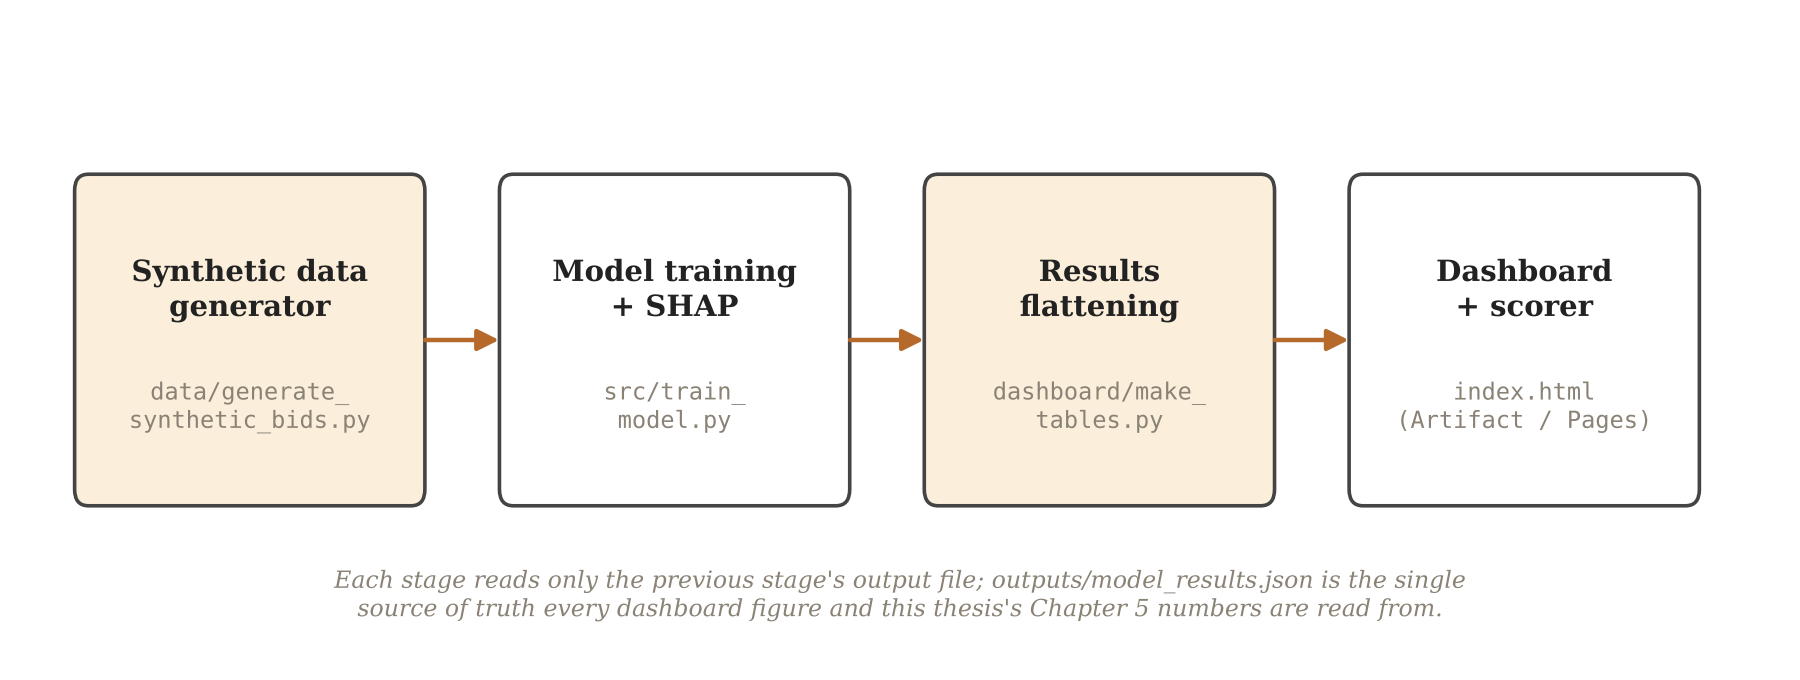
\includegraphics{figures/fig4-1-pipeline-architecture.png}
\caption{The pipeline's four stages, each consuming only the
file the previous stage wrote.}
\end{figure}

Figure 4.1 shows this structure schematically. The shaded stages, data
generation and results flattening, are the two points where the
pipeline's output is reshaped into a different data representation
(synthetic bids into a CSV log; the single nested results file into the
nine flat tables the Claude Artifact dashboard requires, discussed in
Section 4.3); the unshaded stages, model training and the dashboard
itself, are the points where that data is consumed to produce new
information rather than merely reformatted. This distinction matters for
where a future extension of the pipeline, for example the Random
Forest/XGBoost comparison recommended in Chapter 7, would be inserted:
it replaces logic inside the second stage only, and because every later
stage reads only that stage's output file rather than depending on how
the file was produced, no other stage needs to change to accommodate a
different model being trained there.

\hypertarget{data-generation-and-feature-engineering}{%
\section{Data Generation and Feature
Engineering}\label{data-generation-and-feature-engineering}}

\texttt{data/generate\_synthetic\_bids.py} implements the methodology
set out in Chapter 3: five hundred bids are generated with a fixed
random seed for reproducibility. Categorical fields (client segment,
project type, incumbency position) are drawn from fixed marginal
probability distributions chosen to resemble a plausible BU bid log, for
example client segment is drawn as 30\% AAA publisher, 32\% mid-size
publisher, 28\% indie studio, and 10\% platform holder. Correlated
fields are drawn conditionally: deal origin's inbound probability
depends on relationship history; pre-proposal engagement's probability
depends on both deal origin and relationship history; price position is
drawn as a function of project effort plus independent noise, so that
larger engagements receive a small realistic discount on average.

The latent win propensity is computed as a weighted sum of each
feature's encoded effect (the weights, described fully in Chapter 3, are
derived from the Engineering BU's documented hypotheses), plus the three
deliberate interaction terms and the Gaussian noise term, passed through
a logistic transform, with the model's intercept calibrated by binary
search so the realised win rate lands close to the 30\% target. Label
noise is then applied by flipping a random 5\% of outcomes. The
resulting dataset achieved, on this run, a realised win rate of 30.6\%
across the five hundred bids, close to the 30\% target, which confirms
the intercept calibration behaved as intended.

Feature engineering for modelling purposes is comparatively light,
consistent with the dataset having been generated directly in a
model-ready shape: the thirteen raw features are split into ten numeric
fields and three categorical fields (client segment, project type,
incumbency), numeric fields are median-imputed and categorical fields
are imputed with their most frequent value, and categorical fields are
one-hot encoded. This preprocessing is implemented once, as a shared
scikit-learn \texttt{ColumnTransformer}, and reused identically for the
held-out test split, the 5-fold cross-validation, and the full-data SHAP
and scorer training, so that no inconsistency can creep in between these
three uses of the same preprocessing logic.

\hypertarget{model-training}{%
\section{Model Training}\label{model-training}}

The primary predictive model is a scikit-learn
\texttt{GradientBoostingClassifier} (Section 2.2; Friedman
\citeyearpar{friedman2001greedy}), trained with 100 trees, a learning
rate of 0.04, a maximum tree depth of 2, a minimum of 20 samples per
leaf, and 0.8 subsampling per tree. These hyperparameters were chosen
specifically to regularise the model against overfitting on a dataset of
only 500 rows and thirteen features: shallow trees (depth 2) and a
conservative learning rate keep any single tree from fitting noise, the
minimum-leaf-size constraint prevents trees from isolating individual
training examples, and subsampling introduces additional variance
reduction in the spirit of Breiman's \citeyearpar{breiman2001random}
bagging argument, applied here inside a boosting framework. An initial,
less regularised configuration (150 trees, learning rate 0.07, depth 3)
was tried first and produced a visibly larger gap between
cross-validated and held-out performance, a classic overfitting
signature on a dataset this size; the final, more conservative
hyperparameters were selected specifically to close that gap, and
Chapter 5 reports the resulting, more stable performance.

The model is evaluated two ways. A single stratified 75/25 train/test
split (375 training bids, 125 held-out test bids, stratified to preserve
the approximately 30\% win rate in both splits) gives a one-shot
estimate of performance on genuinely unseen data. A separate 5-fold
stratified cross-validation, refitting the full preprocessing-and-model
pipeline on each fold independently to avoid any leakage between folds,
gives a more stable estimate averaged across five different train/test
partitions. Both are reported in Chapter 5, with the cross-validated
figure treated as the more reliable headline number precisely because it
is not sensitive to which 125 bids happened to land in a single test
split.

\hypertarget{shap-explanation-pipeline}{%
\section{SHAP Explanation Pipeline}\label{shap-explanation-pipeline}}

SHAP values are computed using the \texttt{shap} package's
\texttt{TreeExplainer}, applied to a gradient-boosted model refit on the
full five-hundred-bid dataset (a separate fit from the train/test-split
model used for performance evaluation, since the explanation pipeline's
purpose is to characterise what the full available data says about
feature importance, not to avoid leakage in the way a performance
estimate must). \texttt{TreeExplainer} computes exact Shapley values for
tree ensembles in polynomial time, as described in Section 2.3,
returning one signed contribution per model input feature (after one-hot
encoding) for every one of the 500 bids.

Two aggregation steps turn this raw, per-encoded-column output into the
business-readable form the artefact displays. First, one-hot-encoded
columns belonging to the same original categorical feature (for example,
the four \texttt{client\_segment\_*} columns) are summed back into a
single contribution for that feature, so that ``client segment'' appears
once in the global ranking and in each per-bid explanation, rather than
as four separate, harder-to-read partial contributions. Second, the
global feature-importance ranking is computed as the mean absolute SHAP
value for each feature across all 500 bids, a standard global-importance
summary that treats positive and negative contributions symmetrically (a
feature that strongly pushes some bids toward a win and others toward a
loss is still an important feature, even though its \emph{signed}
average contribution might be small). This global ranking is the object
compared against the BU's documented hypothesis ranking (RQ1), using
Spearman's rank correlation coefficient, computed over all thirteen
features; Chapter 5 reports the result and discusses the specific
features where the two rankings diverge most.

For per-bid explanation, eight bids are sampled from the dataset (a
fixed random seed, so the same eight bids appear in the artefact on
every pipeline run) and, for each, the top three positive and top three
negative SHAP contributions (again aggregated to the original feature
level) are extracted alongside the bid's predicted win probability, its
actual recorded outcome, and its full raw feature values. The artefact's
``Example Bids'' section (Section 4.3) displays these eight bids
directly, letting a reader see not only that the model predicted, say, a
70\% win probability, but which specific features drove that number up
or down for that specific bid, and what the bid's full feature profile
actually was.

\hypertarget{the-interactive-dashboard}{%
\section{The Interactive Dashboard}\label{the-interactive-dashboard}}

The dashboard is implemented twice from the same
\texttt{outputs/model\_results.json} source, once as a Claude Artifact
(a shareable, hosted web page with an interactive-dashboard runtime) and
once as a static site published via GitHub Pages, so that the artefact
can be opened either as a quick shareable link or as a permanent,
self-hosted page with no dependency on a third-party hosting platform.
Both versions render the same content from the same underlying numbers;
they differ only in how that data is loaded (the Claude Artifact version
reads from small, per-section JSON datasets attached to the artefact's
own data store, a constraint of that hosting platform that required
restructuring the single nested \texttt{model\_results.json} file into
nine flat, tabular files, one per dashboard section, since that
platform's dashboard type only accepts row-array, not nested-object,
data; the GitHub Pages version fetches the same flat JSON files directly
over HTTP) and in minor styling (each uses its host's own design-token
system for colours, fonts, and spacing, so the dashboard looks native to
wherever it is opened).

The dashboard presents five sections, in order: a synthetic-data
disclaimer banner, stated up front rather than buried in a footnote,
repeating the caveat from Chapter 3 in plain language so that nobody
reading only the artefact, without this thesis, mistakes its numbers for
findings about real Virtuos bids; a model-performance section showing
the 5-fold cross-validated and held-out AUC, the Brier score, the
Spearman rank correlation, the ROC curve, and the confusion matrix, each
accompanied by a short plain-language explanation of what the metric
actually measures rather than only its name and value, since an early
version of the artefact that showed bare metric names and numbers was
judged, during review, to assume more statistical background than its
intended BU audience should need; a global SHAP feature-importance bar
chart; a table comparing the SHAP ranking against the BU's documented
hypothesis ranking, with each feature's rank shift highlighted; and the
eight example bids described above, each with an expandable panel
showing its full feature values alongside its top SHAP factors. Every
feature name in the dashboard, in the SHAP chart, the hypothesis table,
the example-bid detail panels, and the scorer described next, carries a
small clickable control that opens a short, plain-language definition of
that feature, since several of the raw feature names (for example,
``incumbency'') are internal modelling shorthand that a non-technical BU
stakeholder should not be expected to already know.

\hypertarget{the-interactive-what-if-scorer-design-and-the-case-for-a-surrogate-model}{%
\section{The Interactive What-If Scorer: Design and the Case for a
Surrogate
Model}\label{the-interactive-what-if-scorer-design-and-the-case-for-a-surrogate-model}}

RQ3 calls for an artefact a BU stakeholder can use directly, not only
read, and the most direct way to satisfy that for a bid-competitiveness
tool is to let a user describe a hypothetical bid, varying its client
segment, relationship history, price position, and so on, and see an
estimated win probability update live, together with the factors driving
that estimate. This component, the scorer, is the thesis's most concrete
demonstration step in Peffers et al.'s \citeyearpar{peffers2007design}
DSR process.

Implementing the scorer directly against the gradient-boosted model
described above would require evaluating a 100-tree ensemble inside the
browser every time a user moves a slider. This is technically possible,
trees can be serialised and walked in JavaScript, but it was judged to
add real implementation complexity and a real risk of subtle bugs (an
incorrectly ported split condition, for example, would silently produce
wrong probabilities with no obvious symptom) for a component where the
thesis's actual design requirement is a different property: that every
factor the scorer displays be an \emph{exact}, auditable contribution to
the predicted probability, not an approximation and not a black box,
however faithfully implemented.

A logistic regression gives this property directly and exactly, because
its decision function is linear in the standardised input features. A
second model, a scikit-learn \texttt{LogisticRegression} with its
numeric features standardised (zero mean, unit variance) and its
categorical features one-hot encoded, was therefore trained on the full
dataset specifically for the scorer, using the same preprocessing logic
as the gradient-boosted model. For this surrogate model, each feature's
contribution to the predicted log-odds is exactly that feature's
coefficient multiplied by its standardised value, a single
multiplication the browser performs directly from the model's stored
coefficients, with no server round-trip and no approximation. The
scorer's ``top factors'' display is therefore not an estimate of what
mattered; it is the literal arithmetic the probability was computed
from, shown back to the user.

This substitution is made transparent in the artefact itself rather than
hidden: the scorer section states plainly that it runs a linear
surrogate rather than the gradient-boosted model used for the
dashboard's headline performance and SHAP figures, and reports the
surrogate's own performance (an AUC of 0.773 on the full dataset and
0.743 under 5-fold cross-validation) so a user can judge how much
predictive power, if any, is traded away for that exactness. That the
surrogate's cross-validated AUC (0.743) is close to the gradient-boosted
model's cross-validated AUC (reported in full in Chapter 5) indicates
the trade-off is modest for this particular dataset, though this is not
guaranteed to hold in general and is noted as a limitation in Chapter 6:
a future real-data deployment of this scorer should re-check whether a
linear surrogate remains an adequate approximation of the primary
model's behaviour, or whether the interaction effects the
gradient-boosted model can capture (Section 2.2) make that trade-off
larger on real bid data.

\hypertarget{summary}{%
\section{Summary}\label{summary}}

The complete pipeline, shown in Figure 4.1, runs synthetic data
generation, grounded in the BU's documented hypotheses and designed
against trivial circularity; a regularised gradient-boosted classifier,
evaluated both on a held-out split and by cross-validation; a SHAP
explanation layer providing both global feature ranking and per-bid
attribution; and a two-part artefact, a results dashboard and a live,
exactly-auditable scorer built on a transparent logistic surrogate,
published in two independently hosted forms. Chapter 5 now evaluates
each of these components against the research questions set out in
Chapter 1.

\hypertarget{evaluation}{%
\chapter{Evaluation}\label{evaluation}}

This chapter reports the evaluation set out in Chapter 3: quantitative
performance of the gradient-boosted model, the global and per-bid SHAP
results, the SHAP-versus-hypothesis comparison central to RQ1,
evaluation of the scorer's logistic surrogate, and a structured
assessment of the artefact against RQ3. Every figure reported here is
read directly from the pipeline's own output file
(\texttt{outputs/model\_results.json}), consistent with the ``single
source of truth'' design described in Chapter 4; none is recomputed or
adjusted for presentation.

\hypertarget{quantitative-model-performance}{%
\section{Quantitative Model
Performance}\label{quantitative-model-performance}}

The gradient-boosted classifier was evaluated on a held-out test split
(125 of the 500 bids, stratified to preserve the 30.6\% realised win
rate) and separately by 5-fold stratified cross-validation across all
500 bids. Table 5.1 reports both.

\textbf{Table 5.1: Model performance}

\begin{longtable}[]{@{}ll@{}}
\toprule\noalign{}
Metric & Value \\
\midrule\noalign{}
\endhead
\bottomrule\noalign{}
\endlastfoot
Held-out test AUC (single 75/25 split) & 0.632 \\
5-fold cross-validated AUC (mean) & 0.705 \\
5-fold cross-validated AUC (standard deviation) & ± 0.052 \\
5-fold AUC, individual folds & 0.748, 0.674, 0.692, 0.632, 0.776 \\
Brier score (held-out test set) & 0.2103 \\
\end{longtable}

The 5-fold cross-validated AUC of 0.705 is the more reliable headline
figure, since it averages over five different train/test partitions
rather than depending on which 125 bids happened to land in a single
held-out split; the single-split test AUC of 0.632 sits within the range
spanned by the individual cross-validation folds (0.632 to 0.776), so it
is a plausible, if somewhat pessimistic, draw from the same underlying
distribution rather than evidence of a separate problem. Read against
the logistic-regression ceiling established in Chapter 3 (an AUC of
approximately 0.72 for a simple linear baseline on this same data), the
gradient-boosted model's cross-validated AUC of 0.705 is close to,
essentially at, that ceiling. This is a meaningful result in both
directions: it confirms the synthetic dataset carries genuine, learnable
signal rather than being unlearnable noise, and it indicates that, on
this dataset and with the hyperparameters selected in Chapter 4, the
additional non-linear modelling capacity of a gradient-boosted ensemble
over a plain logistic regression is not translating into a materially
higher ceiling, a finding discussed further in Chapter 6.

The Brier score of 0.2103 measures how close the model's predicted
probabilities are to the actual outcomes, averaged over the test set,
where 0 is a perfect forecast and 0.25 is what a model achieves by
always predicting the dataset's base win rate (approximately 30\%)
regardless of any feature. A Brier score of 0.21, modestly below that
0.25 naive baseline, indicates the model is extracting some genuine
probability-calibration benefit from the features, though the margin is
not large, consistent with the AUC result above.

\begin{figure}
\centering
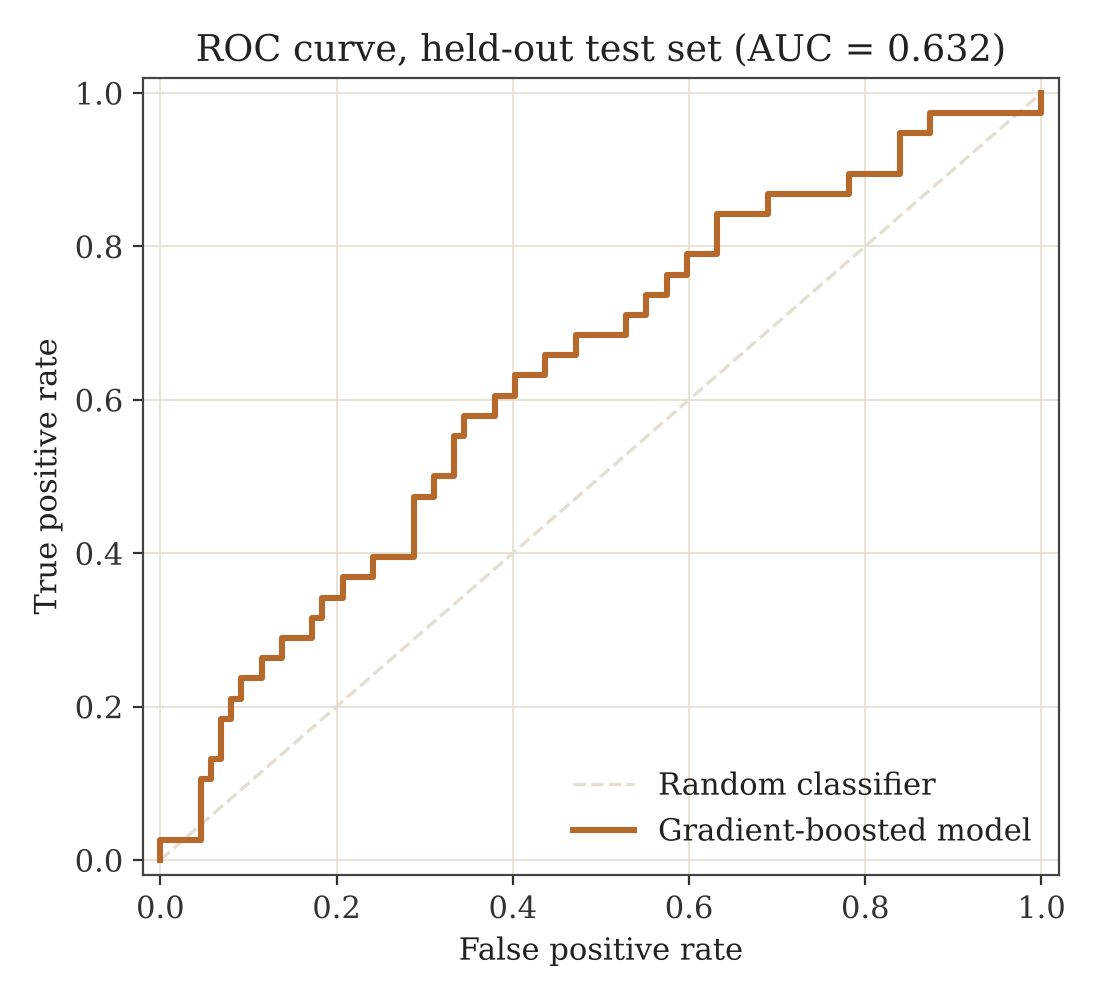
\includegraphics{figures/fig5-1-roc-curve.png}
\caption{ROC curve for the gradient-boosted model on the
held-out test set.}
\end{figure}

Figure 5.1 plots the ROC curve the test-set AUC in Table 5.1 is computed
from. Its shape is informative beyond the single summary number: the
curve sits consistently above the diagonal across almost the entire
false-positive-rate range rather than only in one region, which
indicates the model's ranking ability is reasonably uniform rather than
concentrated at one end of the probability scale (for example, being
good only at confidently identifying the most obviously winnable bids
while offering no real separation among the rest). The step-like shape
is a direct consequence of the test set's modest size (125 bids); with
only 38 actual wins to rank against 87 actual losses, each individual
bid's position in the model's probability ordering moves the curve by a
visible, discrete step, and a larger real-data test set would be
expected to produce a visibly smoother curve at the same underlying AUC.

\hypertarget{confusion-matrix-and-derived-classification-metrics}{%
\subsection{Confusion Matrix and Derived Classification
Metrics}\label{confusion-matrix-and-derived-classification-metrics}}

Table 5.2 reports the confusion matrix at the default 0.5 classification
threshold on the held-out test set, together with the classification
metrics it implies.

\textbf{Table 5.2: Confusion matrix and derived metrics (held-out test
set, n = 125, threshold = 0.5)}

\begin{longtable}[]{@{}lll@{}}
\toprule\noalign{}
& Predicted Lost & Predicted Won \\
\midrule\noalign{}
\endhead
\bottomrule\noalign{}
\endlastfoot
\textbf{Actual Lost} (n = 87) & 77 (true negative) & 10 (false
positive) \\
\textbf{Actual Won} (n = 38) & 28 (false negative) & 10 (true
positive) \\
\end{longtable}

\begin{longtable}[]{@{}ll@{}}
\toprule\noalign{}
Metric (Won class) & Value \\
\midrule\noalign{}
\endhead
\bottomrule\noalign{}
\endlastfoot
Accuracy & 0.696 \\
Precision & 0.500 \\
Recall & 0.263 \\
F1-score & 0.345 \\
\end{longtable}

\begin{figure}
\centering
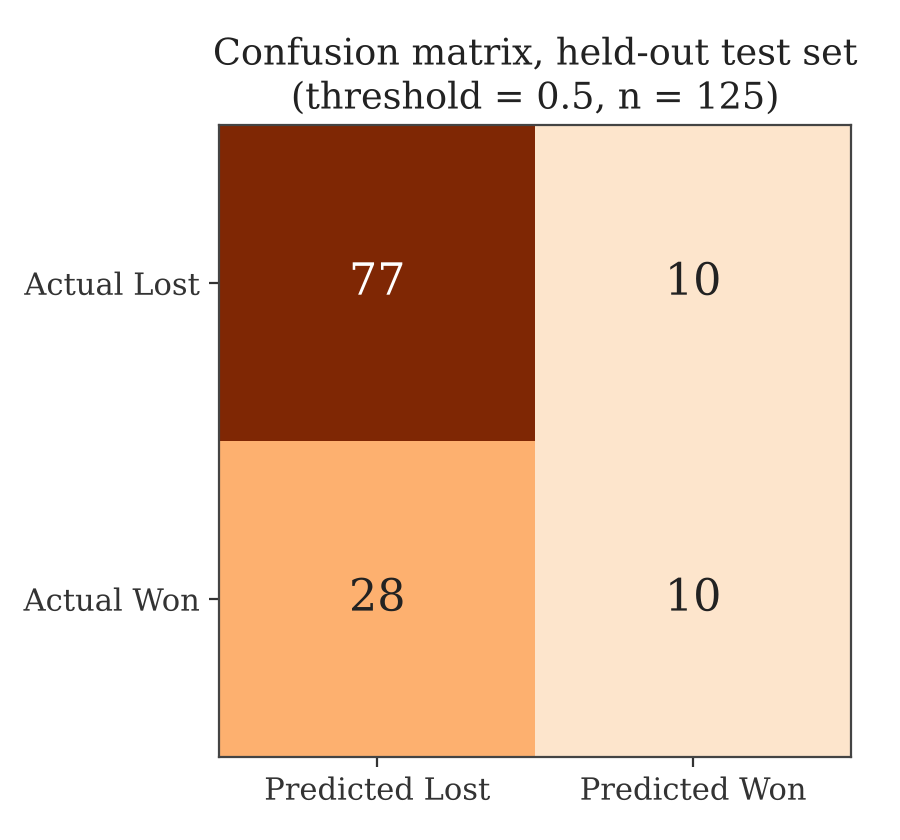
\includegraphics{figures/fig5-3-confusion-matrix.png}
\caption{Confusion matrix at the default 0.5 threshold.}
\end{figure}

Figure 5.2 renders Table 5.2 as a heatmap, which makes the asymmetry
between the two error types visually immediate in a way the table's
numbers alone require a moment's arithmetic to notice: the
false-negative cell (28, bids the model wrongly calls Lost) is nearly
three times the size of the false-positive cell (10, bids the model
wrongly calls Won). This asymmetry is the same class-imbalance effect
discussed below, shown here as a shape rather than only as a derived
recall figure.

The most important pattern in Table 5.2 is the gap between precision
(0.500) and recall (0.263) for the Won class: of the 38 bids the test
set actually recorded as won, the model's default 0.5-threshold
prediction correctly flags only 10, missing 28. This is a direct,
expected consequence of class imbalance (He and Garcia
\citep{he2009learning}, Section 2.1): with a base win rate of roughly
30\%, a threshold of 0.5 is conservative relative to the base rate, and
the model, like most classifiers trained under imbalance without
explicit reweighting, tends to under-predict the minority class at that
threshold even when, as the AUC result shows, it ranks genuinely
winnable bids above genuinely losing ones reasonably well. This is
precisely why AUC, a threshold-independent ranking measure, is reported
as the primary performance figure in Table 5.1 rather than accuracy or
the default-threshold F1-score: a BU stakeholder using this tool in
practice would not be bound to the 0.5 threshold, and could instead
choose a lower threshold (flagging more bids as ``competitive'' at the
cost of more false positives) depending on how the BU wants to trade off
pursuing more opportunities against spending more proposal effort on
bids that ultimately lose. This threshold-selection trade-off is not
resolved by this thesis and is identified in Chapter 7 as a concrete
next step for making the tool more directly actionable.

\hypertarget{global-shap-feature-importance}{%
\section{Global SHAP Feature
Importance}\label{global-shap-feature-importance}}

Table 5.3 reports the full global SHAP ranking, computed as the mean
absolute SHAP value per feature across all 500 bids (Chapter 4).

\begin{figure}
\centering
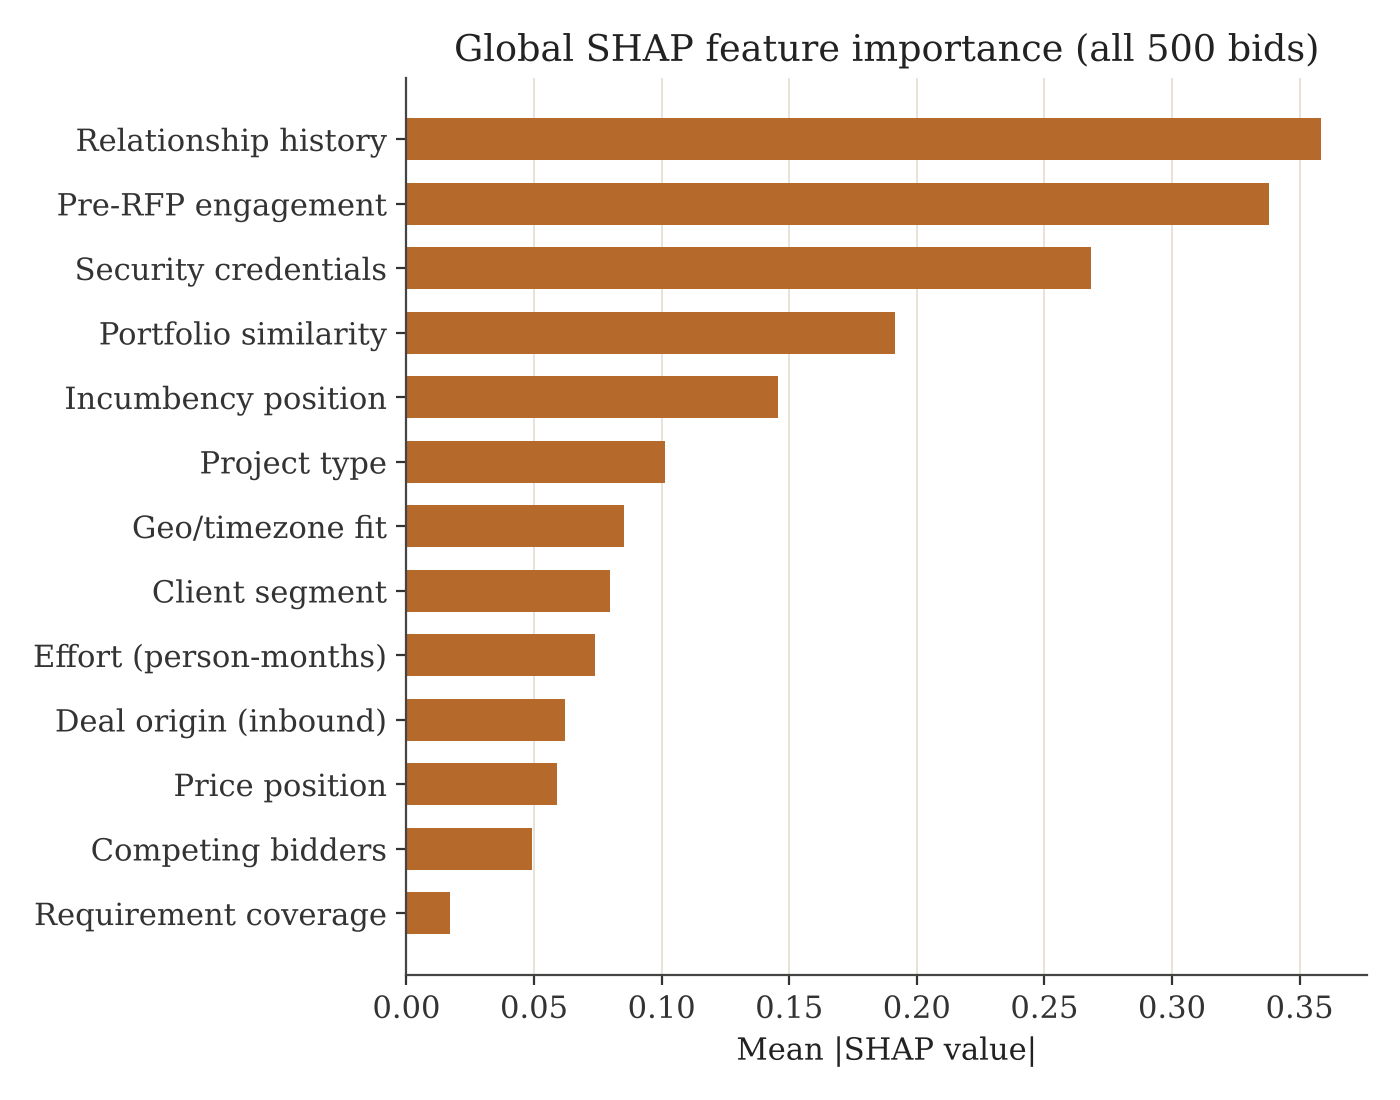
\includegraphics{figures/fig5-2-shap-importance.png}
\caption{Global SHAP feature importance, all thirteen
features, sorted.}
\end{figure}

Figure 5.3 plots the same ranking as Table 5.3. Read as a shape rather
than as thirteen individual numbers, it shows a visible break after the
fifth feature (security credentials, at 0.2683): the top five features
cluster at values from roughly 0.15 to 0.36, then the remaining eight
drop to a comparatively flat band under 0.10, with only a gentle decline
from one to the next. This two-tier structure is itself a finding worth
reporting independently of the exact rank ordering within either tier:
it suggests the model's predictions are driven predominantly by a small
core of five features, with the remaining eight contributing real but
comparatively minor and more interchangeable signal, a pattern
consistent with the data generator's own design (Chapter 3), where a
smaller number of features carry deliberately larger encoded weights and
three specific interaction terms are concentrated among this same top
tier (relationship history, pre-RFP engagement, security credentials,
and portfolio similarity all appear in at least one of the three encoded
interactions).

\textbf{Table 5.3: Global SHAP feature importance (all 500 bids)}

\begin{longtable}[]{@{}lll@{}}
\toprule\noalign{}
Rank & Feature & Mean \\
\midrule\noalign{}
\endhead
\bottomrule\noalign{}
\endlastfoot
1 & Relationship history & 0.3585 \\
2 & Pre-RFP engagement & 0.3379 \\
3 & Security credentials & 0.2683 \\
4 & Portfolio similarity & 0.1916 \\
5 & Incumbency position & 0.1456 \\
6 & Project type & 0.1015 \\
7 & Geo/timezone fit & 0.0854 \\
8 & Client segment & 0.0796 \\
9 & Effort (person-months) & 0.0738 \\
10 & Deal origin (inbound) & 0.0623 \\
11 & Price position & 0.0589 \\
12 & Competing bidders & 0.0492 \\
13 & Requirement coverage & 0.0169 \\
\end{longtable}

Relationship history emerges as the single most influential feature,
consistent with its encoded effect size in the data generator (Chapter
3) and with the general finding in the win-propensity literature that
prior relationship is a strong predictor of future outcomes (Yan et al.
\citeyearpar{yan2015sales}; Rezazadeh
\citeyearpar{rezazadeh2020generalized}). Pre-RFP engagement and security
credentials rank second and third, both plausible on their face, early
engagement shapes a proposal to a client's actual needs, and security
credentials gate entry for the AAA-publisher and platform-holder
segments specifically, which is exactly the interaction effect
deliberately encoded into the data generator (Chapter 3). That this
interaction surfaces as a high global-importance feature, rather than
being invisible to a method that only reports average effects, is a
point in favour of the pipeline correctly recovering a non-additive
relationship, though confirming the \emph{interaction} specifically,
rather than only the feature's overall importance, would require
inspecting SHAP interaction values or a segment-conditioned breakdown,
which this thesis's current evaluation does not include and which is
identified in Chapter 7 as a specific next step.

\hypertarget{rq1-shap-ranking-against-the-bus-documented-hypotheses}{%
\section{RQ1: SHAP Ranking Against the BU's Documented
Hypotheses}\label{rq1-shap-ranking-against-the-bus-documented-hypotheses}}

Table 5.4 reports the full comparison between the Engineering BU's
documented hypothesis ranking (the order features were expected to
matter in, before any modelling) and the rank SHAP actually assigns each
feature after training.

\textbf{Table 5.4: BU hypothesis rank versus SHAP rank, by feature}

\begin{longtable}[]{@{}llll@{}}
\toprule\noalign{}
Feature & BU hypothesis rank & SHAP rank & Shift \\
\midrule\noalign{}
\endhead
\bottomrule\noalign{}
\endlastfoot
Relationship history & 1 & 1 & No change \\
Deal origin (inbound) & 2 & 10 & Down 8 \\
Pre-RFP engagement & 3 & 2 & Up 1 \\
Requirement coverage & 4 & 13 & Down 9 \\
Incumbency position & 5 & 5 & No change \\
Portfolio similarity & 6 & 4 & Up 2 \\
Price position & 7 & 11 & Down 4 \\
Geo/timezone fit & 8 & 7 & Up 1 \\
Security credentials & 9 & 3 & Up 6 \\
Competing bidders & 10 & 12 & Down 2 \\
Effort (person-months) & 11 & 9 & Up 2 \\
Client segment & 12 & 8 & Up 4 \\
Project type & 13 & 6 & Up 7 \\
\end{longtable}

The Spearman rank correlation between the two orderings is
\textbf{0.242}. Read in isolation, this is a weak positive correlation,
and it is worth restating the methodological caveat from Chapter 3
explicitly here: because the synthetic data generator's encoded weights
were themselves derived from this same BU hypothesis document, a
\emph{much} higher correlation would have been the more naively expected
outcome, and the fact that it is not near 1.0 is not, by itself, a sign
that the pipeline failed. Three features account for most of the
divergence and are each individually explicable rather than symptomatic
of a broken pipeline.

\textbf{Security credentials (hypothesis rank 9, SHAP rank 3, up 6).}
The data generator encodes a strong \emph{interaction} effect for this
feature, specifically for AAA-publisher and platform-holder clients,
security credentials matter substantially more than their flat,
segment-independent effect alone would suggest. The BU's hypothesis
ranking, by construction, ranks features on their expected flat
importance; SHAP's mean-absolute-value summary, by contrast, captures
the feature's importance averaged across all the conditions it appears
in, including the specific client segments where its effect is
amplified. A feature whose importance is concentrated in a subset of
cases, rather than spread evenly, can rank much higher in a SHAP summary
than in a simple a priori importance guess that does not anticipate that
interaction. This is, in the author's reading, the pipeline correctly
surfacing a pattern the flat hypothesis ranking was not designed to
anticipate, rather than a failure to recover the hypothesis.

\textbf{Requirement coverage (hypothesis rank 4, SHAP rank 13, down 9)
and deal origin (hypothesis rank 2, SHAP rank 10, down 8).} These are
the two largest downward shifts, features the BU expected to matter
considerably more than SHAP finds they do. Requirement coverage's
encoded effect in the data generator is comparatively modest relative to
several other features (Chapter 3), and its values are also fairly
tightly clustered around the dataset's mean (Appendix A), which limits
how much variation in predicted probability it can account for even if
its per-unit effect were otherwise large; a feature with a real but
narrow range of observed values will tend to show a smaller
mean-absolute-SHAP contribution than one with the same per-unit effect
but a wider observed range, simply because SHAP measures realised
contribution across the actual data, not a feature's theoretical maximum
influence. Deal origin's downward shift is smaller in absolute SHAP
terms but large in rank terms specifically because several features
cluster closely around similarly modest importance values in the bottom
half of Table 5.3, where small differences in mean
\textbar SHAP\textbar{} translate into comparatively large rank
movements. Both cases illustrate a general, useful methodological point
for RQ1: a rank-based comparison like this one is sensitive to
clustering in the underlying importance values in a way that comparing
the raw importance scores directly is not, and a fuller evaluation
(identified in Chapter 7) would report both the rank comparison and the
underlying score differences side by side.

\textbf{Project type (hypothesis rank 13, SHAP rank 6, up 7).} This is
the largest upward shift and the converse of the security-credentials
case: a feature the BU's flat hypothesis ranked as least important turns
out to carry real signal once the model has access to the rest of the
feature set, plausibly because project type correlates with several
other features (effort, portfolio similarity) in ways the generator's
correlation structure (Chapter 3) builds in deliberately, so part of
what SHAP attributes to ``project type'' may be signal that is genuinely
shared with those correlated features rather than independent to project
type alone. Disentangling shared, correlated signal from each individual
feature's independent contribution is a known general limitation of SHAP
and of feature-importance methods more broadly, and is noted as such in
Chapter 6 rather than treated as specific to this result.

Taken together, these three cases support treating the overall finding
of RQ1 as follows: the model's two highest-ranked features by the BU's
own hypothesis (relationship history and incumbency position) are
recovered at identical rank by SHAP, which is a meaningful, direct
confirmation at the top of the ranking; the correlation across the full
ranking is weak rather than strong, which, given the interaction effects
and value-range differences discussed above, is judged to be an
interesting and explicable methodological result rather than evidence
the pipeline failed to recover the encoded signal, but which does mean
this thesis cannot claim the pipeline reproduces the BU's full
hypothesis ordering faithfully, only its top end and its broad logic.

\hypertarget{per-bid-explanation-qualitative-review-of-example-bids}{%
\section{Per-Bid Explanation: Qualitative Review of Example
Bids}\label{per-bid-explanation-qualitative-review-of-example-bids}}

The eight example bids the artefact displays (Chapter 4) were reviewed
qualitatively against their SHAP explanations and full feature profiles.
In general, the explanations are internally coherent: bids with high
predicted win probability (for example, the first example bid, an
AAA-publisher live-ops proposal predicted at 70.3\% and actually won)
are consistently explained by positive contributions from pre-RFP
engagement, security credentials, and portfolio similarity, each a
top-ranked global feature in Table 5.3; bids with low predicted win
probability (for example, an indie-studio co-development proposal
predicted at 9.7\% and actually lost) are consistently explained by
negative contributions from relationship history, portfolio similarity,
and pre-RFP engagement, the same top features acting in the opposite
direction. This consistency between a bid-level explanation and the
global ranking is expected, since both are computed from the same
underlying SHAP values, but confirming it holds in practice, rather than
only in aggregate, is exactly what the per-bid explanation view is for,
and this review found no example among the eight where the stated top
factors were inconsistent with the bid's actual feature values.

The deliberately non-monotonic encoded pattern described in Chapter 3,
that a prior client whose delivery went poorly is encoded as
\emph{worse} for win probability than a brand-new client, was not
directly testable from the current evaluation output: the pipeline
reports an aggregate SHAP importance for ``relationship history'' as a
whole but does not currently export a per-level breakdown (the
contribution specifically at level 1, ``prior, poor delivery,'' versus
level 0, ``new client'') that would show whether the model separated
these two levels correctly rather than treating relationship history as
a simple monotonic scale. This is flagged here as a specific, known gap
in the current evaluation rather than glossed over: Chapter 7 recommends
adding a partial-dependence or SHAP-dependence plot for this feature
specifically as a near-term extension, since it is the one deliberately
designed test case in the synthetic data (Chapter 3) that this thesis's
evaluation does not yet directly confirm or disconfirm.

\hypertarget{evaluation-of-the-scorers-logistic-surrogate}{%
\section{Evaluation of the Scorer's Logistic
Surrogate}\label{evaluation-of-the-scorers-logistic-surrogate}}

The logistic-regression surrogate that drives the artefact's interactive
scorer (Chapter 4) achieves an AUC of 0.773 on the full dataset and
0.743 under 5-fold cross-validation (standard deviation 0.048). The
cross-validated figure is the more reliable one for the same reason
given in Section 5.1, and it sits close to, if marginally above, the
gradient-boosted model's own cross-validated AUC of 0.705. This is a
favourable result for the design choice made in Chapter 4: the scorer
trades the gradient-boosted model's modest additional ranking power for
an exact, auditable client-side computation, and on this dataset that
trade costs little to nothing in predictive performance, within the
noise of a 500-row dataset.

This favourable result should not be over-read as evidence that a linear
model is generally sufficient for this problem; Chapter 3's generator
deliberately encodes non-linear interaction effects specifically to
motivate using a tree-based learner at all (Section 2.2), and a logistic
model, by construction, cannot represent those interactions directly,
only indirectly, to the extent a feature's main effect correlates with
the interaction's net impact across the dataset. The more precise
reading is that, on \emph{this} dataset's realised noise level and
sample size, the gap between a model that can represent interactions and
one that cannot happens to be small; whether that remains true on a
larger, real dataset, where interaction effects might be both stronger
and more precisely estimable, is explicitly left open and flagged in
Chapter 6 as a limitation of the scorer specifically, distinct from the
dashboard's primary model.

\hypertarget{rq3-structured-evaluation-of-the-artefact}{%
\section{RQ3: Structured Evaluation of the
Artefact}\label{rq3-structured-evaluation-of-the-artefact}}

RQ3 asks how the dashboard and scorer convert the model's output into
usable decision-support information, and what building the artefact
reveals about the practical requirements for deploying a tool like this.
This thesis evaluates that question structurally, against four concrete
requirements implied by RQ3's own wording, rather than through a formal
user study, which was out of scope (Section 1.6) given the absence of
real bid data and real BU users to test against.

\textbf{Does the artefact present model output without requiring
statistical background?} The performance-metric explanations added to
each stat tile (Chapter 4), stating in plain language what AUC, the
Brier score, and the Spearman correlation each actually measure, and the
clickable feature-definition system covering every technical or
internal-shorthand feature name, were both added specifically in
response to this requirement, after an earlier version of the artefact
that displayed bare metric names and raw feature keys was judged, in
review, to assume a BU stakeholder already knew what an AUC or an
``incumbency'' field meant. This is treated as a positive, if informally
evaluated, result: the requirement was identified as unmet and then
concretely addressed.

\textbf{Does the artefact let a user see why, not only what?} The SHAP
chart, the hypothesis-comparison table, and each example bid's
top-factor breakdown jointly satisfy this for the dashboard's
retrospective, aggregate view; the scorer's live, exact factor breakdown
satisfies it for a hypothetical, forward-looking bid a user constructs
themselves. Both views are backed by the same underlying explanation
method applied to two different models, which is disclosed explicitly in
the artefact (Chapter 4) rather than left for a careful reader to
notice.

\textbf{Is the artefact actually usable without a licensing or access
barrier?} This was the central reason for the Power BI-to-web-dashboard
deviation (Chapter 3), and the resulting artefact, openable in any
browser with no account or license required, directly satisfies this
requirement in a way the originally proposed Power BI delivery would not
have, for any reviewer or BU stakeholder without an existing Power BI
license.

\textbf{What did building the artefact reveal about deployment
requirements that the original design did not anticipate?} Two concrete
findings from the implementation process are reported here because they
bear directly on this part of RQ3. First, the Claude Artifact hosting
platform's dashboard type only accepts flat, tabular (row-array) data
from an attached file, not the nested JSON structure
\texttt{outputs/model\_results.json} naturally has; this was discovered
only when the first version of the dashboard loaded with no data at all,
and required restructuring the pipeline's output into nine separate flat
tables (Chapter 4) before the artefact would render. This is a concrete,
generalisable lesson for any future deployment of this pipeline to a
similar dashboard platform: the data-shape constraints of the chosen
hosting mechanism should be checked before, not after, the results
file's structure is finalised. Second, the decision to build the scorer
on a separate, explicitly linear surrogate model, rather than on the
primary gradient-boosted model, was not part of the original design and
emerged specifically from the tension between wanting exact, auditable
explanations and wanting to avoid porting a tree ensemble into
JavaScript; this is reported as a genuine, unplanned design finding from
the DSR process's demonstration step (Peffers et al.
\citeyearpar{peffers2007design}), not as a decision made in advance.

\hypertarget{summary-against-the-research-questions}{%
\section{Summary Against the Research
Questions}\label{summary-against-the-research-questions}}

RQ1 is answered with a specific, evidenced result rather than a simple
yes or no: the model's top two features by the BU's own hypothesis are
recovered at identical SHAP rank, and the largest divergences are each
individually explicable (an interaction effect surfacing a feature's
importance above its flat expectation; a narrow observed value range
understating a feature's realised contribution; correlated signal being
partly attributed to a feature the flat hypothesis under-weighted), but
the overall rank correlation (0.242) is weak, and this thesis does not
claim the pipeline faithfully reproduces the BU's full hypothesis
ordering. RQ2 is answered with a cross-validated AUC of 0.705, close to
the dataset's own logistic-regression ceiling of approximately 0.72,
indicating the gradient-boosted model recovers close to the full
recoverable signal in this synthetic data but gains comparatively little
from its additional non-linear capacity on this specific dataset, a
finding Chapter 6 discusses alongside the dataset-size limitation that
likely drives it. RQ3 is answered structurally: the artefact meets the
four concrete usability requirements derived from the research question,
and the implementation process surfaced two genuine, reportable design
findings, the hosting platform's tabular-data constraint and the case
for a separate scorer model, that were not anticipated in the original
design and are themselves part of this thesis's contribution. Chapter 6
now discusses what these results mean together, their limitations, and
the threats to validity they raise.

\hypertarget{discussion}{%
\chapter{Discussion}\label{discussion}}

This chapter interprets the Chapter 5 results together, sets out the
thesis's limitations and threats to validity in full, and discusses what
the work implies for the Engineering BU in practical terms, distinct
from the strictly evaluative reporting of the previous chapter.

\hypertarget{interpreting-the-results-together}{%
\section{Interpreting the Results
Together}\label{interpreting-the-results-together}}

Three results from Chapter 5, read together rather than individually,
form the thesis's central finding. First, the gradient-boosted model's
cross-validated AUC (0.705) sits close to the dataset's own
logistic-regression ceiling (approximately 0.72), which means the choice
of a non-linear tree ensemble over a simple linear baseline bought
comparatively little on this particular dataset, despite the data
generator deliberately encoding non-linear interaction effects that a
linear model cannot represent directly (Chapter 3). Second, the scorer's
separate logistic surrogate achieved a cross-validated AUC (0.743) that
is, if anything, marginally \emph{higher} than the primary
gradient-boosted model's. Third, the SHAP-versus-hypothesis Spearman
correlation (0.242) is weak despite the two rankings sharing a common
origin by construction.

The most defensible reading of these three results together is that the
dataset, 500 bids, thirteen features, and a true win rate near 30\%, is
simply too small, relative to the number and subtlety of the effects
encoded into it, for a more flexible model to reliably extract
additional signal beyond what a well-regularised linear model already
captures, and for a rank-correlation measure computed over only thirteen
features to settle into a stable, strongly positive value even when the
underlying model is behaving sensibly. This is not a failure of the
pipeline; it is consistent with the general finding in the B2B
win-prediction literature (Section 2.1) that datasets in this domain are
characteristically small and noisy, and it is a genuine, informative
result about what this thesis's synthetic data, deliberately built to be
realistically small and noisy rather than large and clean, can and
cannot show. A real Virtuos bid history, almost certainly larger over
time and subject to a different, organisation-specific noise structure,
may behave differently on both counts, which is precisely why Chapter 7
identifies moving to real data as the priority next step rather than
further tuning this synthetic-data pipeline.

The two visual results reported in Chapter 5, the SHAP ranking's
two-tier structure (Figure 5.3) and the ROC curve's consistent, uniform
separation above the diagonal (Figure 5.1), add a further layer to this
reading rather than standing apart from it. A model whose ranking
ability is spread fairly evenly across the probability scale, rather
than concentrated at one end, and whose predictive signal is
concentrated in a small core of features rather than spread thinly
across all thirteen, is the kind of result a genuinely learnable but
modestly sized problem produces: there is a real, identifiable pattern
(the top-tier features), and the model finds it consistently (the ROC
shape) without needing, or benefiting much from, the full flexibility a
gradient-boosted ensemble offers over the top of that pattern. Put
differently, the ceiling this thesis finds (Section 6.1, first
paragraph) is not a ceiling imposed by an unusually hard or noisy
top-tier signal; it is a ceiling that sits just above where five
features' worth of signal, cleanly separated from the remaining eight,
naturally lands on a dataset this size. This is a specific, testable
prediction for the real-data replication Chapter 7 recommends: if the
same two-tier structure and the same uniform ROC separation reappear on
real bid data, it would suggest the ceiling identified here is a
property of the problem's underlying structure rather than an artefact
of this particular synthetic dataset's construction; if they do not, for
example if a real dataset's SHAP ranking is flatter across all thirteen
features with no clear tier break, that would itself be a finding about
how real bid dynamics differ from the BU's documented hypotheses in a
way this synthetic data, built from those same hypotheses, could not
have anticipated.

\hypertarget{limitations}{%
\section{Limitations}\label{limitations}}

\textbf{The central limitation, repeated here because it governs how
every other result in this thesis should be read, is that the dataset is
synthetic.} Every number reported in Chapter 5, the AUC values, the SHAP
ranking, the hypothesis comparison, is a statement about whether the
pipeline correctly recovers a signal the author encoded, not a statement
about what actually wins real Virtuos bids. This thesis has been
explicit about this distinction throughout (Section 1.6, Chapter 3, and
the artefact's own disclaimer banner), and it is restated here as a
limitation rather than only as a scoping note, because it bounds every
other finding: a reader who takes, for example, ``requirement coverage
ranks low in SHAP importance'' as a real finding about Virtuos's actual
bid dynamics would be misreading this thesis's claim.

\textbf{Dataset size.} Five hundred bids is small by machine-learning
standards generally, and the 5-fold cross-validation's standard
deviation of ± 0.052 around the mean AUC (Table 5.1) is itself evidence
of that: a model's measured performance varies meaningfully depending on
which 100 bids happen to fall in a given validation fold. A real Virtuos
bid history, accumulated over a longer period, would very likely be
larger, which both the literature (Section 2.1) and this thesis's own
cross-validation variance suggest would materially improve the
stability, and plausibly the ceiling, of any model built on it.

\textbf{The two scoping deviations from the original proposal.} Section
3.4 gave the full reasoning for building around a single
gradient-boosted model rather than a Random Forest-versus-XGBoost
comparison, and for a web dashboard rather than Power BI. Both are
reiterated here as limitations rather than neutral choices: RQ2's answer
in this thesis characterises one specific algorithm family's performance
ceiling on this data, not a comparison across families, and the artefact
does not demonstrate Power BI's enterprise deployment features
(row-level security, scheduled refresh against a live source,
integration into an existing BU reporting workspace). Both are treated
in Chapter 7 as concrete, well-defined future work rather than as
abandoned scope, precisely because the pipeline and the structured
results file (Chapter 4) were built in a form that makes both extensions
straightforward to add later without redoing the underlying work.

\textbf{The scorer's surrogate-model trade-off.} Section 5.5 found the
linear surrogate's cross-validated AUC close to, even marginally above,
the primary model's, but cautioned against generalising that result,
since the surrogate cannot represent the interaction effects the data
generator deliberately encodes (Chapter 3), only their average, additive
approximation. Whether this trade-off remains small on a larger, real
dataset, where interaction effects might be more strongly and more
precisely estimable, is not established by this thesis.

\textbf{No formal user study.} RQ3 was evaluated structurally, against
four concrete requirements derived from the research question itself
(Section 5.6), rather than through a study with real BU stakeholders
using the artefact to make real or simulated bid decisions. This was a
necessary consequence of the absence of real bid data and real-decision
context available to this thesis (Section 1.6), but it means the
artefact's usability claims rest on the author's own structured review
rather than on independent evidence from its intended users.

\textbf{Unresolved threshold and loss-reason granularity.} Section 5.1
identified the gap between precision and recall at the default 0.5
threshold as a direct consequence of class imbalance, and noted that a
BU stakeholder could choose a different threshold depending on their
risk tolerance; this thesis does not recommend a specific threshold or
build threshold selection into the artefact. Relatedly, Zahid et al.'s
\citeyearpar{zahid2021predicting} finding that splitting losses into
distinct reasons (no bid, client did not pursue, lost to competition)
adds decision-relevant nuance beyond a flat Won/Lost label was noted in
Chapter 2 but not implemented here; the synthetic data generator and the
model both treat the outcome as strictly binary.

\textbf{The relationship-history non-monotonicity was designed but not
directly confirmed.} As reported in Section 5.4, the pipeline's current
evaluation output does not include a per-level breakdown of the
relationship-history feature's effect, so whether the model specifically
distinguished ``prior client, poor delivery'' from ``new client'' (the
deliberately counter-intuitive pattern described in Chapter 3) rather
than treating the feature as a simple monotonic scale is not established
either way by the current evaluation.

\hypertarget{threats-to-validity}{%
\section{Threats to Validity}\label{threats-to-validity}}

\textbf{Internal validity.} The strongest threat to internal validity in
this thesis is the circularity risk inherent in validating a pipeline
against data the same pipeline's author generated: because the data
generator's weights, the model's training data, and the hypothesis
comparison's reference ranking all trace back to the same source
document (the BU's feature hypotheses), there is a structural risk of
the evaluation confirming what it was built to confirm. This thesis
addresses this risk in two ways rather than denying it exists: the data
generator deliberately introduces noise, interaction effects, and a
non-monotonic pattern specifically so the recovered signal is not a
trivial restatement of the input (Chapter 3), and the
SHAP-versus-hypothesis comparison is reported with its actual, weak
correlation value (0.242) and a candid discussion of why, rather than a
stronger correlation being engineered or implied. The threat is
mitigated, not eliminated; it is eliminated only once the pipeline is
run on real, independently recorded bid data, which this thesis does not
have.

\textbf{External validity.} The results in Chapter 5 generalise, at
most, to the claim that this pipeline's method, synthetic data design,
model training, SHAP explanation, and artefact construction, functions
correctly under the conditions tested. They do not generalise to a claim
about real Virtuos bid dynamics, to other BUs within Virtuos, to other
organisations in the co-development industry, or to other bidding
contexts generally, each of which may have a different, unmodelled
feature set, a different noise structure, and a different true win rate.

\textbf{Construct validity.} The thirteen features used (Chapter 3) are
a reasonable operationalisation of the BU's documented hypotheses, but
they are not a complete account of what might drive a real bid's
outcome; features such as the specific individuals involved, the
detailed technical content of a proposal, or macroeconomic conditions at
the time of bidding are not represented, and a real-data implementation
may find some of these matter more than any feature in the current set.

\textbf{Reliability.} The data generation, train/test split, and
cross-validation fold assignment all use a fixed random seed, so the
specific numbers reported in Chapter 5 are exactly reproducible by
re-running the pipeline (Appendix C gives the exact commands), which
supports this thesis's own internal reliability. It does not, however,
establish that the \emph{qualitative} findings (which features rank
highly, how large the AUC gap between models is) would be robust to a
different random seed; a single run with a different seed could
plausibly shift the cross-validation fold AUCs enough to change, for
example, whether the gradient-boosted model's ceiling reads as ``close
to'' or ``clearly above'' the logistic baseline. This was not tested
across multiple seeds and is noted as a reliability limitation.

\hypertarget{implications-for-the-engineering-bu}{%
\section{Implications for the Engineering
BU}\label{implications-for-the-engineering-bu}}

Read with the limitations above firmly in view, this thesis's practical
implication for the Engineering BU is not ``these are the features that
win bids,'' which the synthetic-data caveat rules out as a claim this
thesis can support, but a narrower, still useful one: a decision-support
pipeline of this shape, data-to-model-to-SHAP-to-artefact, is buildable,
runs end to end on data resembling a real bid log in structure and
scale, and produces output (a global importance ranking, per-bid
explanations, a live scorer) in a form the BU's own stakeholders can
read without statistical training. The concrete next step this implies
for the BU is not to act on any specific feature ranking in Chapter 5,
but to begin systematically recording resolved bid outcomes against this
same thirteen-feature structure, so that this pipeline can be re-run on
real data as soon as a sufficient history exists, an action item made
concrete in Chapter 7's recommendations.

\hypertarget{conclusion}{%
\chapter{Conclusion}\label{conclusion}}

\hypertarget{summary-of-contribution}{%
\section{Summary of Contribution}\label{summary-of-contribution}}

This thesis set out to design, build, and evaluate an end-to-end
decision-support pipeline that predicts the win probability of an
Engineering BU proposal and explains that prediction in a form a
business stakeholder can act on, framed as Design Science Research
\citep{peffers2007design, hevner2004design} and structured internally by
CRISP-DM \citep{chapman2000crispdm}. The delivered contribution has four
parts: a synthetic bid dataset, generated from the Engineering BU's own
documented feature hypotheses and deliberately designed, through noise,
correlation, interaction effects, class imbalance, and a
counter-intuitive encoded pattern, to avoid trivial circularity (Chapter
3); a gradient-boosted classification model, evaluated both on a
held-out split and by cross-validation and found to sit close to the
dataset's own recoverable-signal ceiling (Chapter 5); a SHAP explanation
layer providing both a global feature-importance ranking and per-bid
attribution, including a systematic comparison of that ranking against
the BU's a priori hypotheses (RQ1, Chapter 5); and a two-part
interactive artefact, a results dashboard and a live, exactly-auditable
what-if scorer built on a transparent logistic surrogate, published in
two independently accessible forms (Chapter 4).

Against the three research questions: RQ1 found that the model's
top-ranked features agree with the BU's own top hypotheses, but that the
full ranking correlation is weak (Spearman ρ = 0.242), with the largest
divergences individually explicable through interaction effects,
value-range differences, and correlated signal rather than indicating
pipeline failure. RQ2 found a cross-validated AUC of 0.705, close to the
dataset's logistic-regression ceiling of approximately 0.72, indicating
the pipeline recovers close to the full signal the synthetic data
carries, while leaving open whether a more flexible model's advantage
would be larger on bigger, real data. RQ3 found that the artefact meets
four concrete usability requirements derived from the research question
itself, and that building it surfaced two genuine, unplanned design
findings, a hosting-platform data-shape constraint and the case for a
separate, exactly-interpretable scorer model, that are themselves part
of this thesis's contribution to how this kind of artefact should be
built.

Two deliberate deviations from the thesis's original proposal, a single
gradient-boosted model rather than a Random Forest-versus-XGBoost
comparison, and a web dashboard rather than Power BI, were made explicit
from Chapter 1 onward rather than left for a reader to discover, with
the reasoning for each given in full in Chapter 3 and revisited as
limitations in Chapter 6. Both are treated here not as scope abandoned
but as scope deferred: the pipeline was deliberately built so that both
extensions are straightforward additions to existing, working
infrastructure rather than work that must start from nothing.

\hypertarget{recommendations-for-future-work}{%
\section{Recommendations for Future
Work}\label{recommendations-for-future-work}}

\textbf{Move to real bid data.} This is the single highest-priority next
step and the one every other recommendation below depends on for its
real-world relevance. The Engineering BU should begin recording resolved
bid outcomes against the thirteen-feature structure used in this thesis
(Chapter 3), so that the existing pipeline, the data preparation, model
training, SHAP explanation, and artefact-generation code, can be re-run
on real data as soon as a sufficient history accumulates, with no change
to the pipeline itself beyond pointing it at a new input file. A
realistic minimum sample size to begin with should be judged against the
± 0.052 cross-validation variance this thesis found on 500 synthetic
bids (Chapter 5); a real dataset of a similar or larger size would be a
reasonable first target.

\textbf{Run the originally proposed Random Forest-versus-XGBoost
comparison.} Because the synthetic data, feature engineering, and
evaluation harness built for this thesis already exist and are reusable,
adding Random Forest \citep{breiman2001random} and XGBoost
\citep{chen2016xgboost} as additional candidate models and comparing all
three on the same held-out split and cross-validation folds is a
well-defined, comparatively low-effort extension, and should be the
first modelling change made once real data is available, both because it
restores the thesis's original scope and because the comparison itself
may behave differently on larger, real data than the literature review's
general expectation (Section 2.2) predicts.

\textbf{Confirm whether the per-level relationship-history pattern was
recovered.} Chapter 5 identified this as a specific, known gap in the
current evaluation: adding a SHAP dependence plot or partial-dependence
analysis for the relationship-history feature specifically, showing its
effect at each of the four ordinal levels rather than only its aggregate
importance, would directly test whether the pipeline recovered the
deliberately non-monotonic pattern (prior-poor-delivery scoring worse
than new-client) that Chapter 3 built into the data specifically to test
this.

\textbf{Port the pipeline's output to Power BI.} Appendix B sets out the
concrete steps: the structured results file
\texttt{outputs/model\_results.json} was deliberately built as a
portable, self-contained export rather than in a format tied to the web
dashboard, specifically so this porting work does not require re-running
the modelling or SHAP pipeline, only building a new presentation layer
against existing output. This would restore the original proposal's
delivery mechanism and additionally demonstrate the enterprise
deployment features (row-level security, scheduled refresh) the current
web artefact does not.

\textbf{Add threshold selection and multi-class loss reasons to the
artefact.} Chapter 6 identified both as unresolved: letting a user
adjust the scorer's classification threshold interactively, rather than
fixing it at 0.5, would make the precision/recall trade-off identified
in Chapter 5 directly actionable rather than only reported; and
extending the outcome label from binary Won/Lost to the three-class
scheme Zahid et al. \citeyearpar{zahid2021predicting} report adding
decision-relevant value (no bid, client did not pursue, lost to
competition) would require a labelled real dataset that records which of
these actually occurred, making it a natural second step once real data
collection (the first recommendation above) is under way.

\textbf{Conduct a user study with Engineering BU stakeholders.} Once
real data and a real-decision context exist, evaluating RQ3 directly,
observing BU stakeholders using the dashboard and scorer to inform an
actual bid decision, would replace this thesis's structural, author-led
evaluation (Section 5.6) with independent evidence of the artefact's
practical usability, and would likely surface further, currently
unanticipated design requirements in the way the hosting-platform
constraint and the scorer-model decision did during this thesis's own
development process (Section 5.6).

\hypertarget{closing-statement}{%
\section{Closing Statement}\label{closing-statement}}

This thesis set out to show that a working, explainable
bid-competitiveness pipeline could be designed, built, and evaluated for
Virtuos' Engineering BU, and to do so honestly about what a pipeline
built on synthetic data, and adapted in two deliberate, disclosed ways
from its original proposal, can and cannot claim. The pipeline and
artefact delivered recover a known, encoded signal correctly under
realistic noise, explain their own predictions in a form a non-technical
stakeholder can use, and are built in a shape that makes the path to
real-data deployment, the next and most important step, a continuation
of this work rather than a restart of it.


\bibliography{references}

\hypertarget{appendices}{%
\chapter*{Appendices}\label{appendices}}
\addcontentsline{toc}{chapter}{Appendices}

\hypertarget{appendix-a-synthetic-data-generation-full-parameters}{%
\section*{Appendix A: Synthetic Data Generation, Full
Parameters}\label{appendix-a-synthetic-data-generation-full-parameters}}
\addcontentsline{toc}{section}{Appendix A: Synthetic Data Generation,
Full Parameters}

This appendix gives the generator's exact parameters, complementing the
methodology and justification given in Chapter 3. The full generator
source is \texttt{data/generate\_synthetic\_bids.py}.

\textbf{Table A.1: Feature marginal distributions}

\begin{longtable}[]{@{}
  >{\raggedright\arraybackslash}p{(\columnwidth - 2\tabcolsep) * \real{0.5000}}
  >{\raggedright\arraybackslash}p{(\columnwidth - 2\tabcolsep) * \real{0.5000}}@{}}
\toprule\noalign{}
\begin{minipage}[b]{\linewidth}\raggedright
Feature
\end{minipage} & \begin{minipage}[b]{\linewidth}\raggedright
Values and probabilities
\end{minipage} \\
\midrule\noalign{}
\endhead
\bottomrule\noalign{}
\endlastfoot
Client segment & AAA publisher 30\%, mid-size publisher 32\%, indie
studio 28\%, platform holder 10\% \\
Project type & Full development 18\%, co-development 34\%, porting 20\%,
live operations 16\%, art services 12\% \\
Relationship history & New client 45\%, prior/poor delivery 10\%,
prior/neutral delivery 22\%, prior/good delivery 23\% \\
Incumbency position & Greenfield 55\%, defending existing work 22\%,
displacing a competitor 23\% \\
\end{longtable}

Deal origin, pre-RFP engagement, effort, price position, requirement
coverage, portfolio similarity, geo/timezone fit, security credentials,
and competing-bidder count are each drawn conditionally or from
continuous distributions (lognormal for effort; Beta for geo/timezone
fit; Poisson for competing bidders) as described in Chapter 3; exact
distributional parameters are given in the generator source.

\textbf{Table A.2: Encoded log-odds weights (relative effect on win
propensity)}

\begin{longtable}[]{@{}
  >{\raggedright\arraybackslash}p{(\columnwidth - 2\tabcolsep) * \real{0.5000}}
  >{\raggedright\arraybackslash}p{(\columnwidth - 2\tabcolsep) * \real{0.5000}}@{}}
\toprule\noalign{}
\begin{minipage}[b]{\linewidth}\raggedright
Feature / level
\end{minipage} & \begin{minipage}[b]{\linewidth}\raggedright
Encoded effect
\end{minipage} \\
\midrule\noalign{}
\endhead
\bottomrule\noalign{}
\endlastfoot
Relationship history: new / poor prior / neutral prior / good prior &
−0.35 / −0.55 / +0.35 / +0.95 \\
Deal origin: inbound & +0.75 \\
Pre-RFP engagement & +0.65 \\
Incumbency: greenfield / defending / displacing & 0 / +0.55 / −0.60 \\
Price position & −0.045 per point above benchmark; −0.017 per point
below \\
Requirement coverage & +2.4 × (coverage − 0.75) \\
Portfolio similarity & +1.3 × (similarity − 0.5) \\
Effort & −0.0012 × (person-months − 90) \\
Geo/timezone fit & +0.9 × (fit − 0.6) \\
Security credentials & +0.20 (base; see interaction below) \\
Competing bidders & −0.12 × (count − 3) \\
Interaction: weak portfolio (\textless{} 0.45) × new client & −1.1 \\
Interaction: security credentials × AAA/platform segment & +0.85 \\
Interaction: price overage × indie-studio segment & −0.03 per point \\
Latent noise & Gaussian, σ = 1.25 \\
Label noise & 5\% of outcomes flipped post-draw \\
\end{longtable}

The intercept is calibrated by binary search so the realised win rate
lands close to 30\%; on the run this thesis reports, the realised win
rate was 30.6\% across 500 bids.

\hypertarget{appendix-b-power-bi-migration-plan}{%
\section*{Appendix B: Power BI Migration
Plan}\label{appendix-b-power-bi-migration-plan}}
\addcontentsline{toc}{section}{Appendix B: Power BI Migration Plan}

This appendix sets out concretely what porting the delivered pipeline's
output to Power BI, the originally proposed delivery mechanism (Section
1.6, Section 3.4), would involve, since the pipeline was deliberately
built to make this a presentation-layer addition rather than a rebuild.

\begin{enumerate}
\def\labelenumi{\arabic{enumi}.}
\tightlist
\item
  \textbf{Data import.} \texttt{outputs/model\_results.json}, or the
  nine flattened per-section tables already generated for the Claude
  Artifact dashboard (\texttt{dashboard/tables/*.json}, Chapter 4),
  would be imported via Power Query as Power BI tables; the flattened
  tables are directly usable as-is, since Power BI, like the Claude
  Artifact platform, works natively with tabular data.
\item
  \textbf{Report pages.} Each dashboard section described in Chapter 4
  maps to one Power BI report page: a performance-summary page (card
  visuals for AUC, Brier score, and the Spearman correlation, plus a
  line chart for the ROC curve and a matrix visual for the confusion
  matrix); a SHAP importance page (a horizontal bar chart); a
  hypothesis-comparison page (a table visual with conditional formatting
  on the rank-shift column); and an example-bids page (a table with
  drill-through to a detail page per bid).
\item
  \textbf{The scorer.} This is the one component that cannot be ported
  directly, since Power BI's native interactivity does not support a
  live, client-side arithmetic scorer in the way the web artefact's
  JavaScript implementation does (Section 4.4). The closest native
  equivalent is a set of Power BI ``What if'' parameters, one slider per
  numeric feature and one dropdown per categorical feature, feeding a
  DAX measure that replicates the logistic surrogate's exact computation
  (intercept plus the sum of each standardised feature times its
  coefficient, passed through a logistic transform), using the
  coefficients already exported in
  \texttt{outputs/model\_results.json}'s \texttt{scorer\_model} object.
  This is a direct, mechanical translation of existing, already-computed
  numbers into DAX, not new modelling work.
\item
  \textbf{Refresh.} A scheduled Power BI refresh, pulling an updated
  \texttt{model\_results.json} each time the underlying pipeline is
  re-run (for example, on a periodic schedule once real bid data
  accumulates, Chapter 7), would restore the MLOps-style automated
  refresh specified in the original proposal, implemented as a scheduled
  task that re-runs \texttt{src/train\_model.py} and republishes its
  output file to wherever Power BI's refresh step reads from.
\end{enumerate}

\hypertarget{appendix-c-repository-and-pipeline-structure}{%
\section*{Appendix C: Repository and Pipeline
Structure}\label{appendix-c-repository-and-pipeline-structure}}
\addcontentsline{toc}{section}{Appendix C: Repository and Pipeline
Structure}

\textbf{Table C.1: Pipeline scripts, their CRISP-DM stage (Chapter 3),
and how to run them}

{\footnotesize
\begin{longtable}[]{@{}
  >{\raggedright\arraybackslash}p{(\columnwidth - 6\tabcolsep) * \real{0.3000}}
  >{\raggedright\arraybackslash}p{(\columnwidth - 6\tabcolsep) * \real{0.1700}}
  >{\raggedright\arraybackslash}p{(\columnwidth - 6\tabcolsep) * \real{0.2300}}
  >{\raggedright\arraybackslash}p{(\columnwidth - 6\tabcolsep) * \real{0.3000}}@{}}
\toprule\noalign{}
\begin{minipage}[b]{\linewidth}\raggedright
Script
\end{minipage} & \begin{minipage}[b]{\linewidth}\raggedright
CRISP-DM stage
\end{minipage} & \begin{minipage}[b]{\linewidth}\raggedright
Output
\end{minipage} & \begin{minipage}[b]{\linewidth}\raggedright
Run
\end{minipage} \\
\midrule\noalign{}
\endhead
\bottomrule\noalign{}
\endlastfoot
\texttt{data/generate\_synthetic\_bids.py} & Data understanding, data
preparation & \texttt{data/synthetic\_bids.csv} &
\texttt{python3\ data/generate\_synthetic\_bids.py} \\
\texttt{src/train\_model.py} & Modelling, evaluation &
\texttt{outputs/model\_results.json} &
\texttt{python3\ src/train\_model.py} \\
\texttt{dashboard/make\_tables.py} & Deployment &
\texttt{dashboard/tables/*.json}, \texttt{docs/data/*.json} &
\texttt{python3\ dashboard/make\_tables.py} \\
\texttt{dashboard/index.html} & Deployment & Claude Artifact dashboard &
Published as a hosted Artifact \\
\texttt{docs/index.html} & Deployment & Static GitHub Pages site &
Served from the repository's \texttt{docs/} folder \\
\end{longtable}
}

\texttt{data/methodology\_synthetic\_data.md} gives the synthetic-data
methodology in its original, standalone form, written before this thesis
and incorporated into Chapter 3. All code is version-controlled in the
project's Git repository alongside this thesis document, consistent with
Hevner et al.'s \citeyearpar{hevner2004design} requirement that the
research process be rigorously and repeatably documented (Chapter 3).

\hypertarget{appendix-d-feature-glossary}{%
\section*{Appendix D: Feature
Glossary}\label{appendix-d-feature-glossary}}
\addcontentsline{toc}{section}{Appendix D: Feature Glossary}

This glossary reproduces, for reference, the plain-language feature
definitions built into the artefact's clickable glossary (Chapter 4),
covering every feature used in modelling.

\begin{longtable}[]{@{}
  >{\raggedright\arraybackslash}p{(\columnwidth - 2\tabcolsep) * \real{0.5000}}
  >{\raggedright\arraybackslash}p{(\columnwidth - 2\tabcolsep) * \real{0.5000}}@{}}
\toprule\noalign{}
\begin{minipage}[b]{\linewidth}\raggedright
Feature
\end{minipage} & \begin{minipage}[b]{\linewidth}\raggedright
Definition
\end{minipage} \\
\midrule\noalign{}
\endhead
\bottomrule\noalign{}
\endlastfoot
History with this client & Whether this client is new to Virtuos, or a
repeat client, and if a repeat client, how the last project went:
poorly, fine, or well. \\
Who started the conversation & Whether the client approached Virtuos
about this opportunity (inbound), or Virtuos pursued the client
(outbound). \\
Talked before the formal bid & Whether Virtuos had conversations with
the client about the project before the official request for proposal
went out. \\
Starting position on this deal & Whether this is a brand-new opportunity
with no prior vendor, work Virtuos is already doing that it is
defending, or work currently done by a competitor that Virtuos is trying
to win away. \\
Project size & The estimated effort for the project, in
person-months. \\
Price vs.~the market rate & How Virtuos's quoted price compares to the
typical rate for similar work; positive means priced above that
benchmark. \\
How much of the brief we covered & The share of the client's stated
requirements that the proposal fully addresses. \\
Relevant past work & How closely Virtuos's existing portfolio matches
the kind of work this project needs. \\
Time zone overlap & How much the working hours of Virtuos's team overlap
with the client's. \\
Security credentials in place & Whether Virtuos already holds the data
and IP security certifications this client's industry typically
requires. \\
Number of competing bidders & How many other studios were bidding for
the same project (flagged in Chapter 3 as a possible real-world leakage
risk, since it is often only known after the decision is made). \\
Type of client & AAA publisher, mid-size publisher, indie studio, or
platform holder. \\
Type of project & Full development, co-development, porting, live
operations, or art services. \\
\end{longtable}


\end{document}
